\section{Selections}
\label{sec:ND280:sel}
The goal of the selection is to map theory interaction modes (e.g. CCQE, CC1$\pi^+$, CC DIS) to ND280 selections, so that theory parameters receive largest constraints from fewest exclusive samples. Equivalent FGD1 and FGD2 selections are separated due to differences in systematics and reconstruction: forward-going tracks emanating in FGD1 leaves a track in FGD1, TPC2, FGD2 and TPC3 so has more hits recorded than the FGD2 equivalence, which only passes through FGD2 and TPC3. Furthermore, FGD2 contains plastic scintillator interleaved with passive water layers whereas FGD1 is fully plastic scintillator. Separating FGD1 and FGD2 also allows constraints on water interactions to come strictly from the FGD2 selections.

The fit bins events in the two reconstructed muon variables \pmu and \cosmu. The muon variables are chosen primarily due to excellent detector resolution of muons and because this is what T2K oscillation analyses observe at \sk. There is ongoing effort to bin in pion variables when such are present (e.g. for CC$1\pi^+$ or CCOther selections), and composite variables in the plane transverse to the neutrino, but these will not be presented here.

The selections are entirely defined by the observed reconstructed event topology of an event in the detector and there is no attempt at correcting for misidentified particles. There is also no attempt to correct for nuclear effects such as final-state-interactions.
\begin{itemize}
\item \textbf{CC$0\pi$}: Events with one negative muon without any charged or neutral pions in the final state. It is developed to contain CCQE and 2p2h events and is the largest sample at ND280. An example event display is shown in \autoref{fig:cc0pi_evtdisplay}. \red{show plots of cross-sections at ND280 from NEUT?}
\begin{figure}[htbp]
	\begin{subfigure}[t]{0.49\textwidth}
		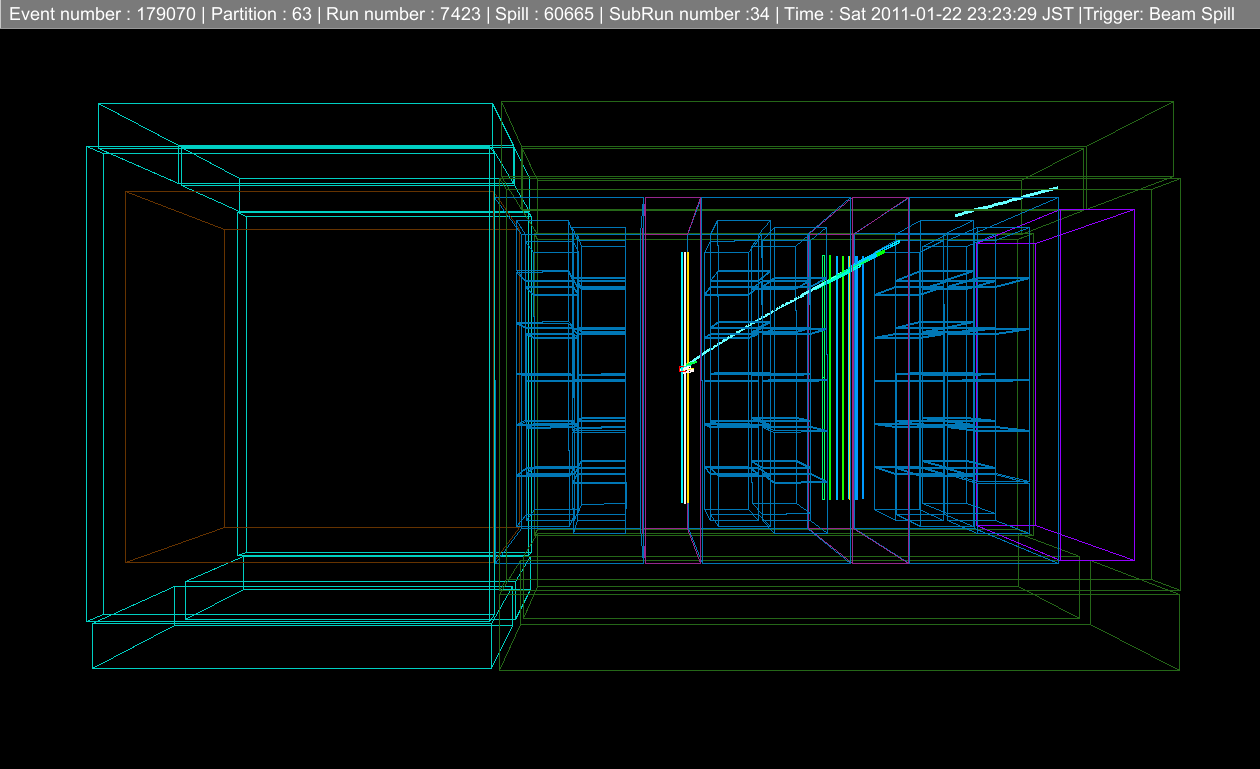
\includegraphics[width=\textwidth, trim={1cm 2.8cm 0 1cm}, clip]{figures/numu/evtdisplay/CC0pi_7423_34_179070_perX0Z_all}
		\caption{Side-view}
	\end{subfigure}
	\begin{subfigure}[t]{0.49\textwidth}
		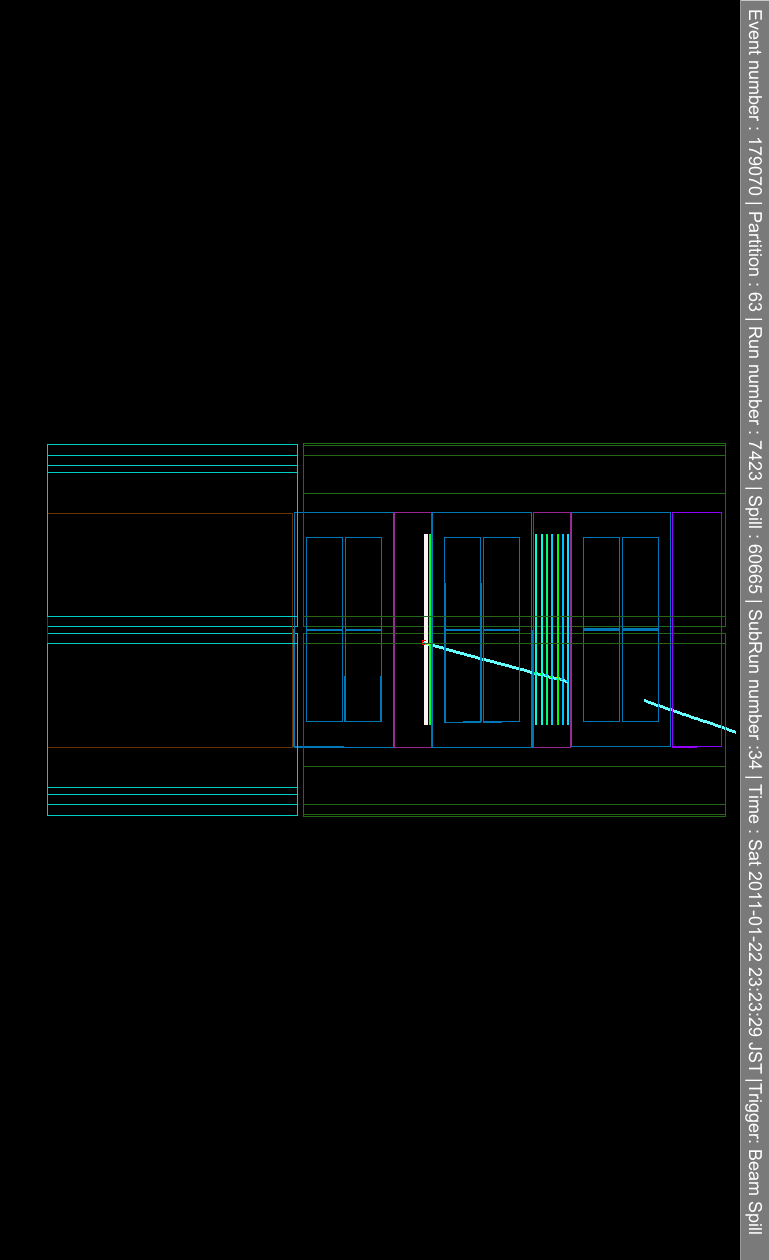
\includegraphics[width=\textwidth, trim={1cm 15cm 1cm 15cm}, clip]{figures/numu/evtdisplay/CC0pi_7423_34_179070_ortX0Z_all}
	\caption{Top-view}
	\end{subfigure}
	\caption{True FGD1 CC0$\pi$ event display in ND280}
	\label{fig:cc0pi_evtdisplay}
\end{figure}

\item \textbf{CC$1\pi$}: Events with one negative muon and one positive pion with no negative or neutral pions in the final state. It is developed to contain mostly CC1$\pi^{+}$ events from resonant interactions\red{refer to previous sections maybe}. An example event display is shown in \autoref{fig:cc1pi_evtdisplay}. 
\begin{figure}[htbp]
	\begin{subfigure}[t]{0.49\textwidth}
		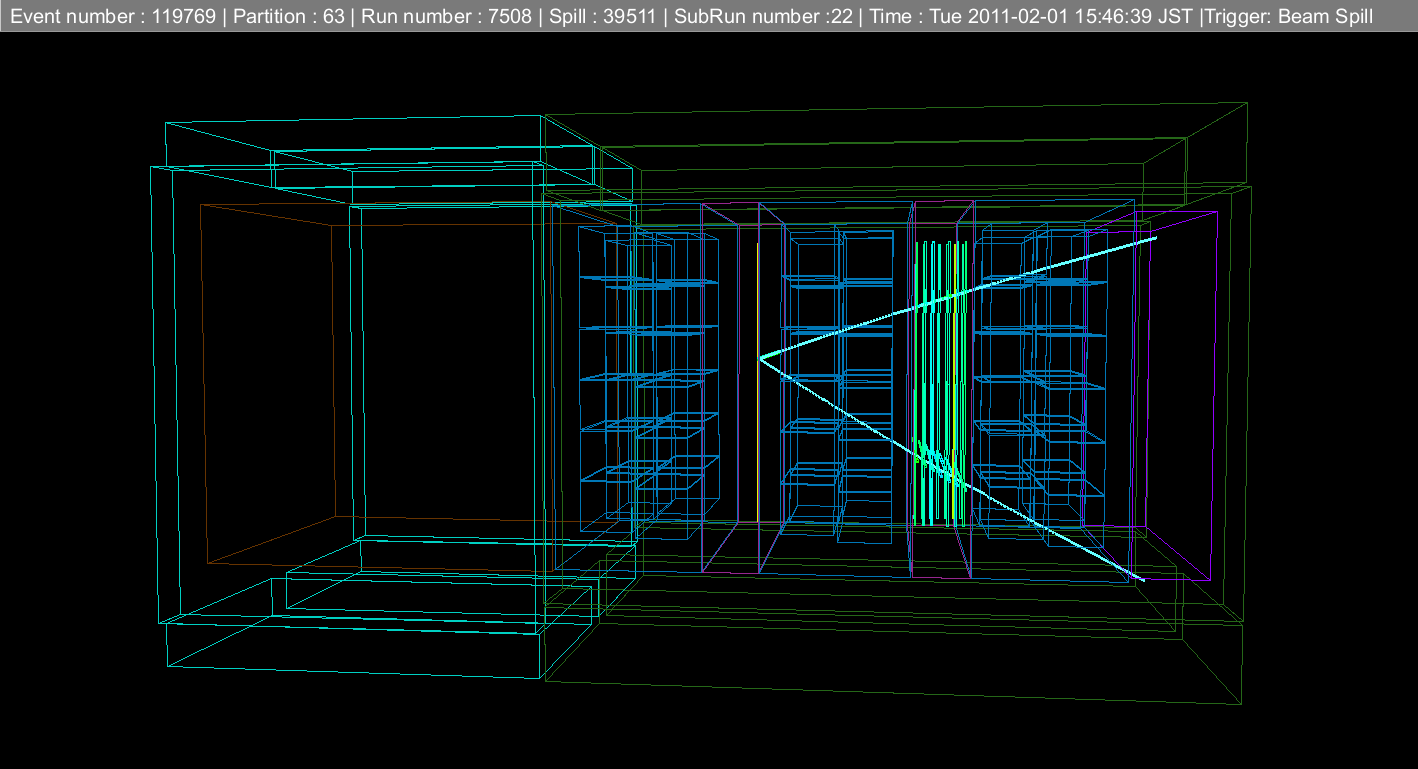
\includegraphics[width=\textwidth, trim={4cm 2cm 4cm 3cm}, clip]{figures/numu/evtdisplay/CC1pi_7508_22_119769_perpX0Z_all}
		\caption{Side-view}
	\end{subfigure}
	\begin{subfigure}[t]{0.49\textwidth}
		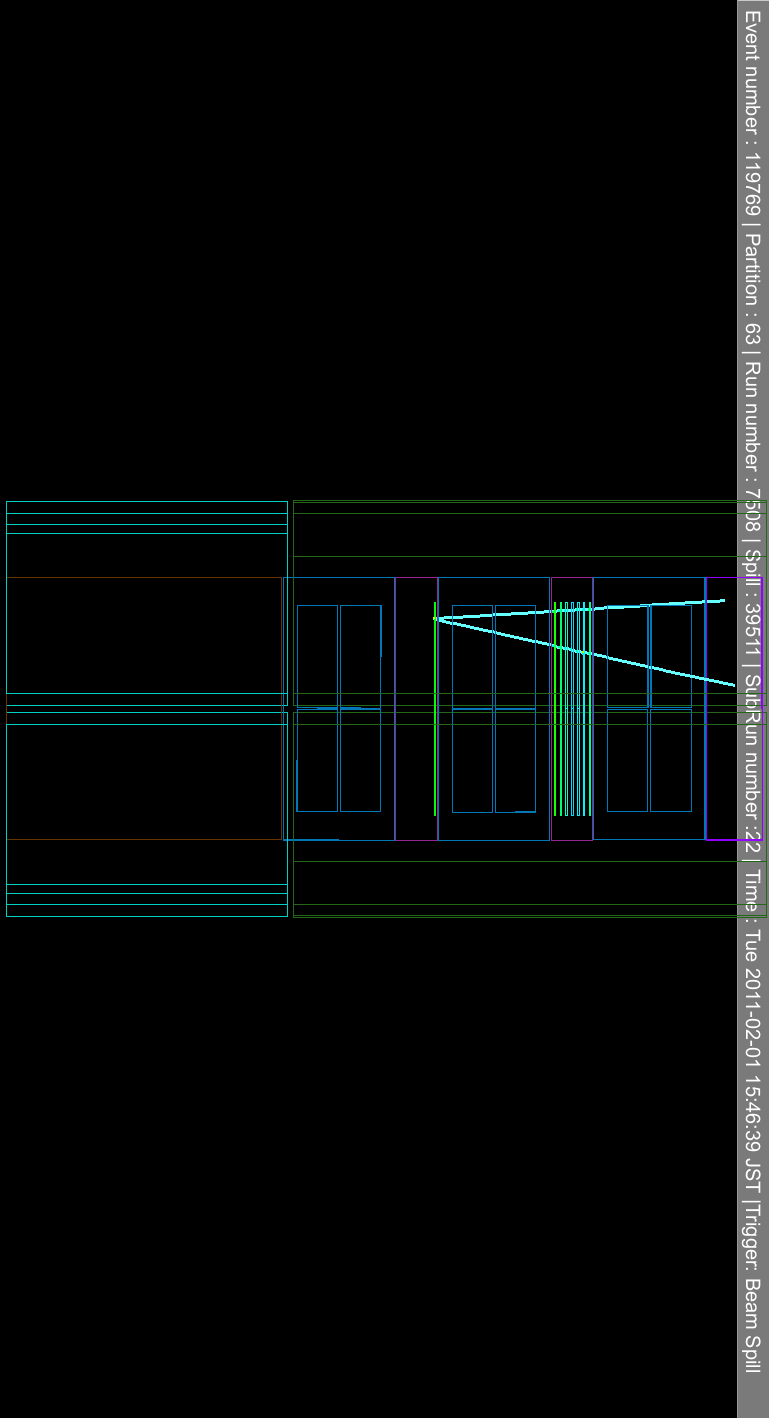
\includegraphics[width=\textwidth, trim={0cm 17cm 1cm 17cm}, clip]{figures/numu/evtdisplay/CC1pi_7508_22_119769_ortX0Z_all}
		\caption{Top-view}
	\end{subfigure}
	\caption{True FGD1 CC1$\pi$ event display in ND280}
	\label{fig:cc1pi_evtdisplay}
\end{figure}

\item \textbf{CC Other}: Events with one negative muon and any number of neutral or negative pions which does not satisfy CC1$\pi$ selection. The presence of one $\pi^{-,0}$ or more than one $\pi^+$ in an event makes this possible. There are no constraints on the number of reconstructed heavier mesons (e.g. kaons or etas). It is developed to contain mostly DIS interactions and CC$1\pi^0$. An example event display is shown in \autoref{fig:ccoth_evtdisplay}.
\end{itemize}
\begin{figure}[htbp]
	\begin{subfigure}[t]{0.49\textwidth}
		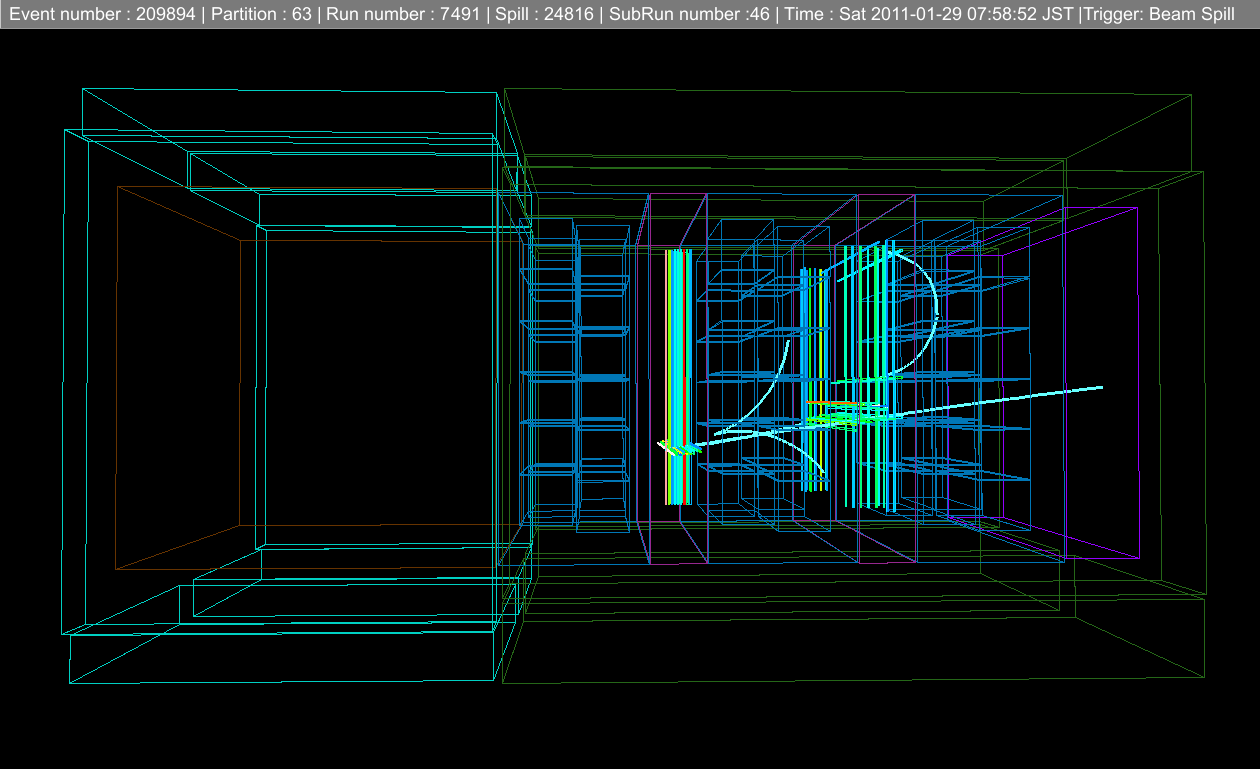
\includegraphics[width=\textwidth, trim={1cm 3cm 1cm 1cm}, clip ]{figures/numu/evtdisplay/CCOthers_7491_46_209894_perX0Z_all}
		\caption{Side-view}
	\end{subfigure}
	\begin{subfigure}[t]{0.49\textwidth}
		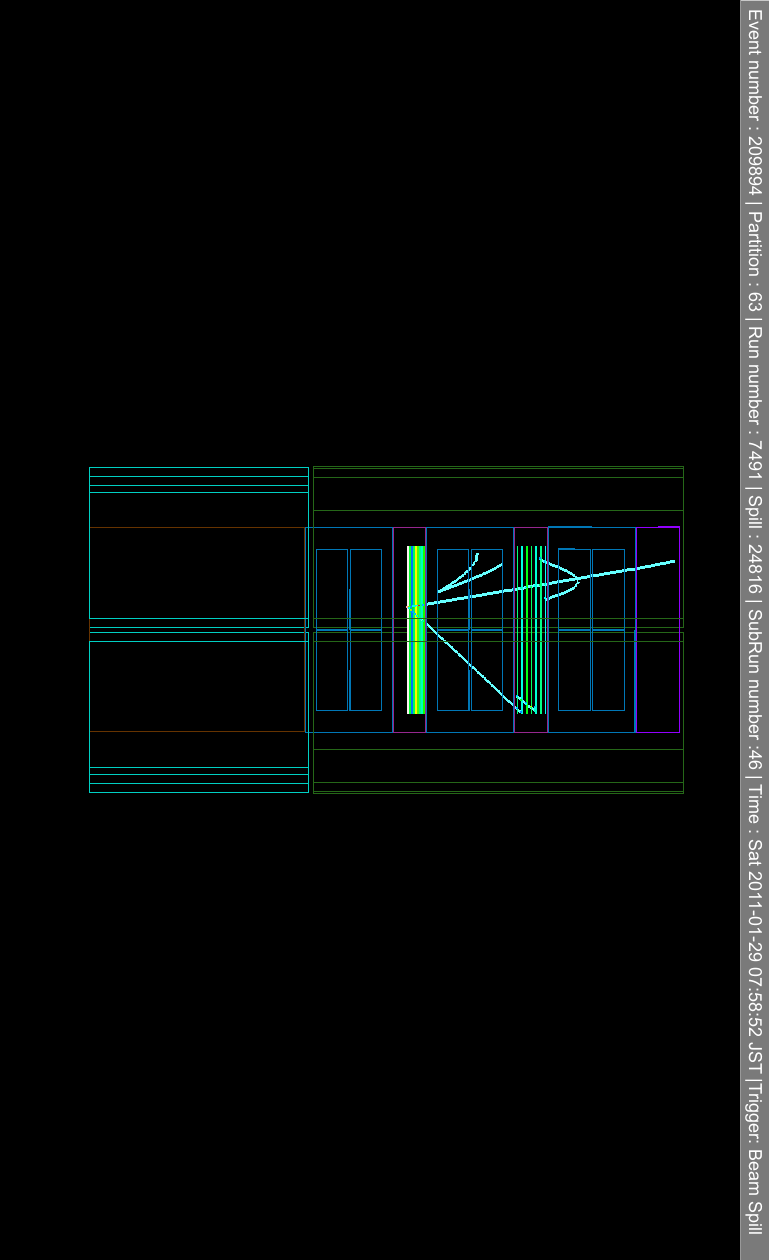
\includegraphics[width=\textwidth, trim={3cm 16cm 3cm 16cm}, clip]{figures/numu/evtdisplay/CCOthers_7491_46_209894_ortX0Z_all}
		\caption{Top-view}
	\end{subfigure}
	\caption{True FGD1 CCOther event display in ND280}
	\label{fig:ccoth_evtdisplay}
\end{figure}

\subsection{Event selection cuts, \numu}
\label{sec:numu_sel}
The different topological selections all start by isolating CC-inclusive candidates in FGD1 or FGD2. Firstly is required to contain one reconstructed track candidate of negative charge crossing the TPC downstream of either FGD (TPC2 for interactions starting in FGD1, TPC3 for interactions starting in FGD2). The event also needs to fulfil data quality and fiducial volume requirements. The muon is then assumed to be the highest momentum negative track (HMNT) found in the event, and it is required that the track is identified as a muon.

The detailed general selection criteria for the CC-inclusive sample is:
\begin{itemize}
	\item \textbf{Event quality cut}: The full beam spill has a good global ND280 data quality flag, meaning all ND280 sub-detectors and magnet were operational and reading out data. The event must occur within the bunch time window of the neutrino beam. Event pile-up is mitigated by associating each event to a beam bunch within a beam spill.
	
	\item \textbf{Quality and fiducial volume cut}: At least one reconstructed track is present in the FGD1 or FGD2 fiducial volume. The fiducial volume for FGD1 is $|x|<874.51\text{ mm}$, $|y-55|<874.51\text{ mm}$, $136.875 < z < 446.955\text{ mm}$ and for FGD2 $|x|<874.51\text{ mm}$, $|y-55|<874.51\text{ mm}$, $1481.45< z < 1807.05\text{ mm}$\footnote{The 55mm offset in $y$ reflects the shift in XY modules relative the center of the ND280 coordinate system.}.
	
	The $x$ and $y$ cuts are designed to accept interactions which have their vertex five bars from the edge of the XY module of each FGD. The $z$ cut excludes the first XY module of each FGD and includes the remaining (14 for FGD1, 7 for FGD2). To reject short tracks, for which the TPC reconstruction is unreliable, tracks are required to have more than 18 TPC clusters.
	
	\item \textbf{Upstream background veto}: If the second highest momentum track starts at least 150 mm upstream of the selected muon candidate (highest momentum negative track with muon PID), the event is rejected. This cut eliminates events in which the muon candidate might be the second part of a broken track which started further upstream (e.g. in the P0D). For events with a reconstructed vertex in FGD2 there is the added criterion of having no reconstructed tracks in FGD1.
	
	\item \textbf{Broken track cut}: The start position of the muon candidate track needs to be less than 425 mm away from the FGD upstream edge if the event has at least one reconstructed FGD-only track. The cut vetoes events where the reconstruction has cut a muon candidate track into two tracks: one of which is fully contained in the FGD and the second starting downstream of the fully contained track in the FGD and enters the TPC, causing the second track to be the selected as the muon candidate, misplacing the vertex.
	
	\item \textbf{Muon PID cut}: Once a particle is considered a muon candidate (fulfilling the above criteria), the particle identification is applied based on the observed $dE/dx$ measurement of the track in the TPC. The measured energy deposit $E$ in the TPC is compared with the expected energy deposit under muon, pion, electron and proton hypotheses and pulls and discrimination functions are then applied.
	
	The pulls $\delta_i$ for particle type $i$ are defined as
	\begin{equation}
	\label{eq:tpc_track_chi2}
	\delta_i = \frac{C_T^{obs}-C_T^{exp}}{\sigma^{exp}}
	\end{equation}
	where the expected energy loss $C_T^{exp}$ is parameterised as
	\begin{equation}
	C_T^{exp} = \frac{53.87 \text{ ADC}}{\beta^{2.283}} \left( 5.551 - \beta^{2.283} - \log\left[0.001913 + \frac{1}{\left(\beta\gamma\right)^{1.249}}\right]\right)
	\end{equation}
	and $\sigma^{exp}$ is the deposited energy resolution of the TPC.
	
	The likelihoods $\mathcal{L}_i$ are then defined as
	\begin{equation}
	\label{eq:tpc_track_likelihood}
		\mathcal{L}_i = \frac{e^{-\delta^2_i}}{\sum_n e^{-\delta^2_n}}
	\end{equation}
	where the denominator is over $n$, which are the particles $n=\mu,\pi,e,p$. 
	
	In the PID algorithm, electrons are rejected by requiring
	\begin{equation}
		\label{eq:tpc_track_mip}
		\mathcal{L}_{MIP} = \frac{\mathcal{L}_\mu + \mathcal{L}_\pi}{1-\mathcal{L}_p} > 0.8
	\end{equation}
	for tracks with $p<500\text{ MeV/c}$. To remove protons and pions, it is required that
	\begin{equation}
	\label{eq:tpc_track_mu}
		\mathcal{L}_\mu > 0.05
	\end{equation}
	The constants 0.8, 0.05 and 500 MeV/c are chosen from particle gun studies in the TPC and test-beam data, and the impact on the selection is shown in \autoref{fig:numu_likelihoods}. The TPC pulls after preselection are shown in \autoref{fig:numu_pulls}, and the energy loss in the TPC from which pulls are derived are shown in \autoref{fig:TPC_dedx}.
	
	Importantly, TPC segments need to pass the TPC track quality cut contribute to the likelihood: bad quality tracks do not. If a track passes through multiple TPCs all TPC tracks are taken into account.
\end{itemize}

\begin{figure}[!h]
	\begin{subfigure}[t]{0.49\textwidth}
		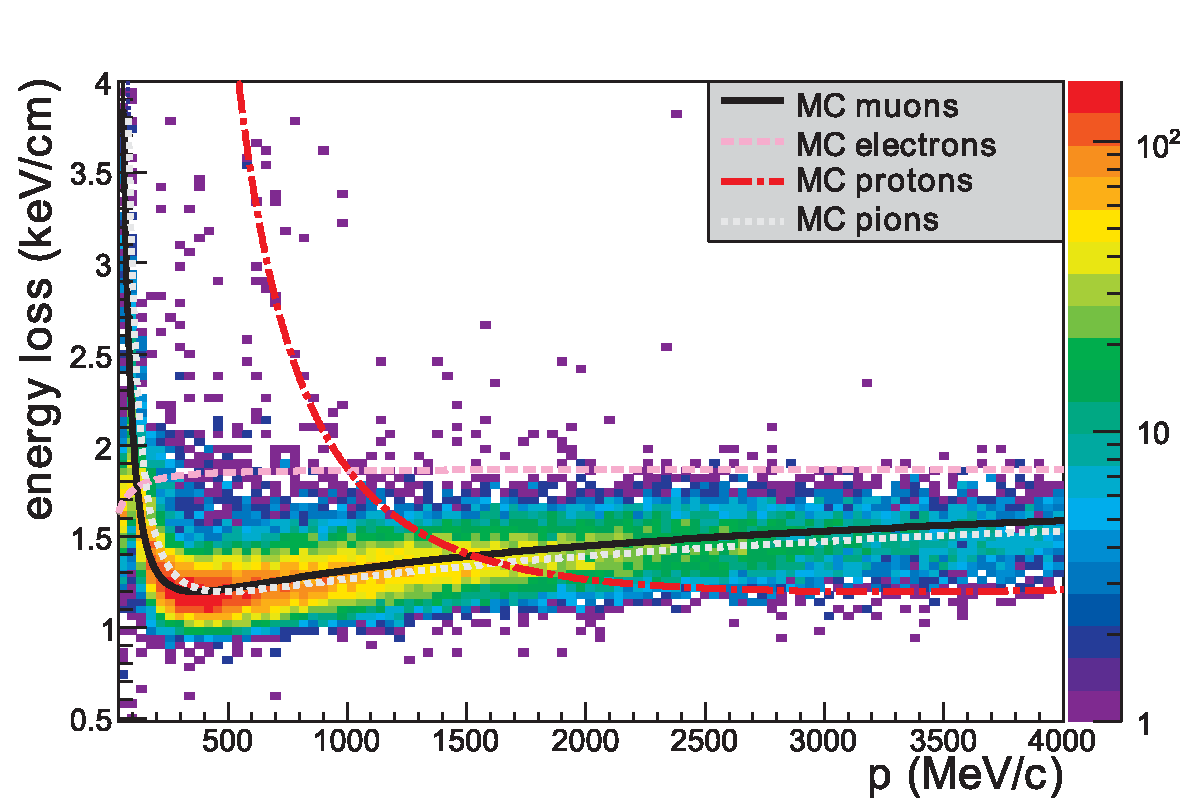
\includegraphics[width=\textwidth]{figures/numu/TPC_PID_neg}
		\caption{Negative particles}
	\end{subfigure}
	\begin{subfigure}[t]{0.49\textwidth}
		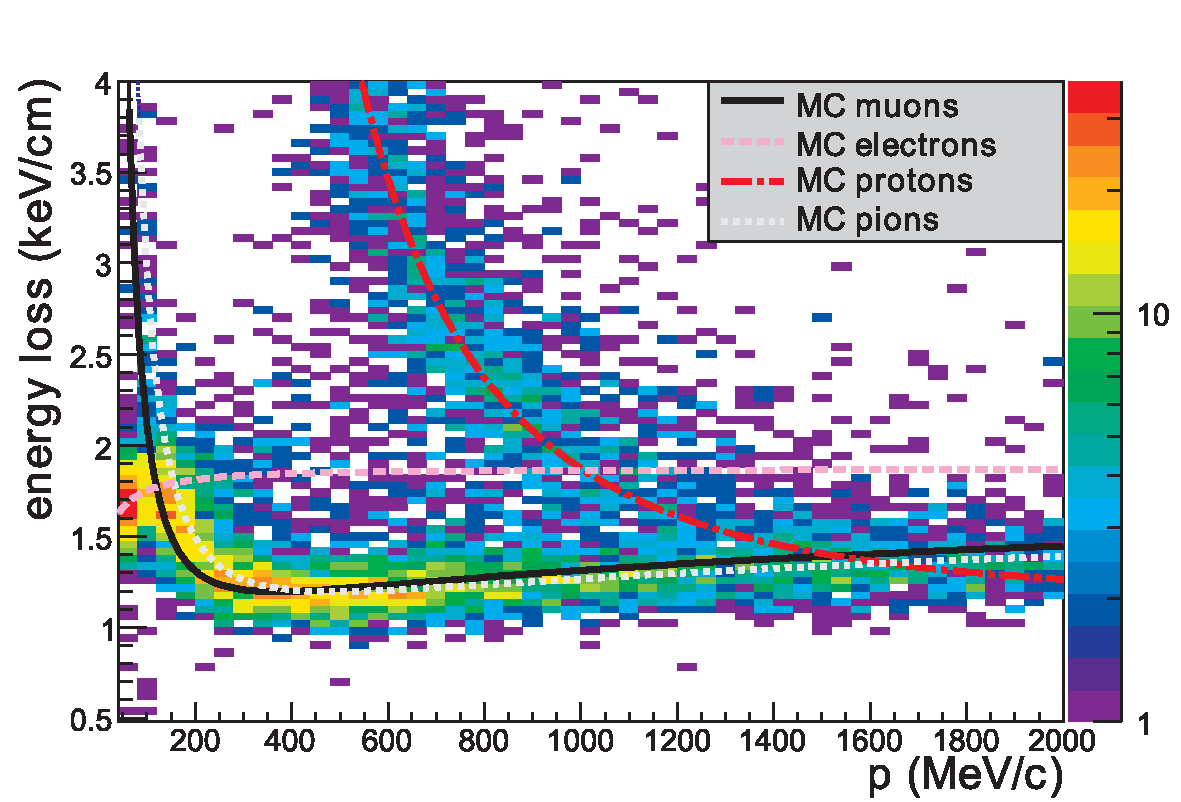
\includegraphics[width=\textwidth]{figures/numu/TPC_PID_pos}
		\caption{Positive particles}
	\end{subfigure}
	\caption{The energy loss for particles travelling through the TPC}
	\label{fig:TPC_dedx}
\end{figure}

\begin{figure}[!h]
	\begin{subfigure}[t]{0.49\textwidth}	
		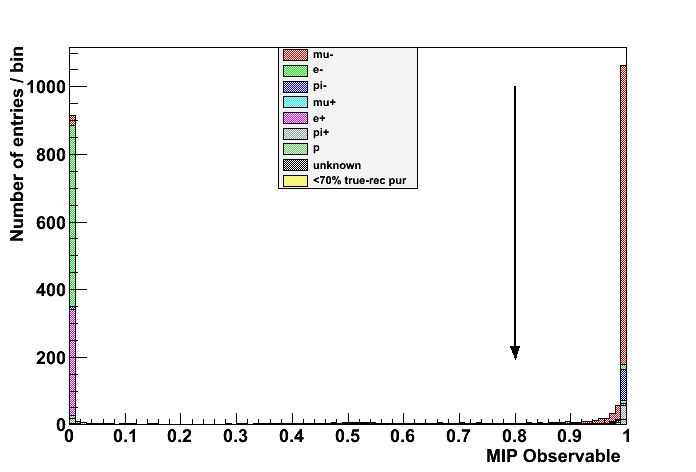
\includegraphics[width=\textwidth]{figures/numu/Cuts/numu/Miplik_run12}
		\caption{$\mathcal{L}_{MIP}$}
	\end{subfigure}
	\begin{subfigure}[t]{0.49\textwidth}	
		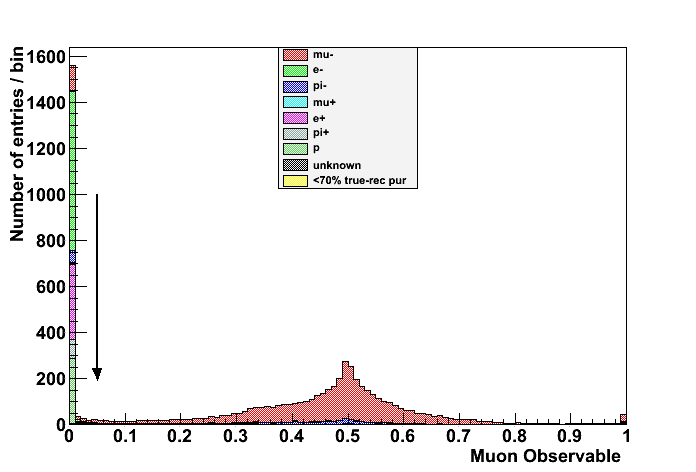
\includegraphics[width=\textwidth]{figures/numu/Cuts/numu/Mulik_run12}
		\caption{$\mathcal{L}_{\mu}$}
	\end{subfigure}
	\caption{Likelihood distributions for preselected MC events, showing cuts placed for \numu analysis}
	\label{fig:numu_likelihoods}
\end{figure}

\begin{figure}[!h]
	\begin{subfigure}[t]{0.32\textwidth}
		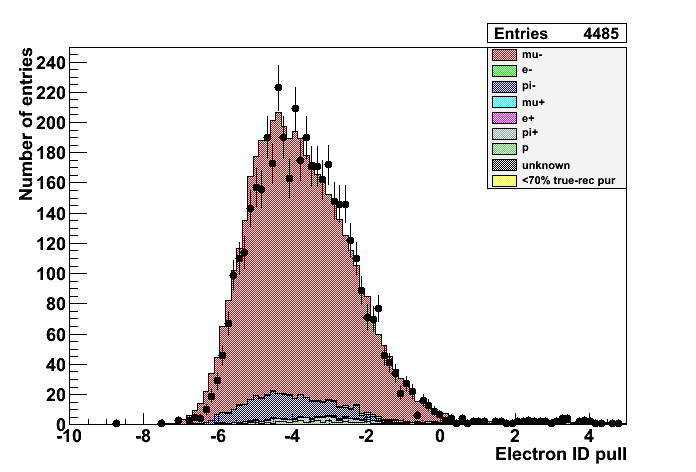
\includegraphics[width=\textwidth]{figures/numu/Cuts/numu/Elepull_run12}
		\caption{$Pull_e$}
	\end{subfigure}
	\begin{subfigure}[t]{0.32\textwidth}	
		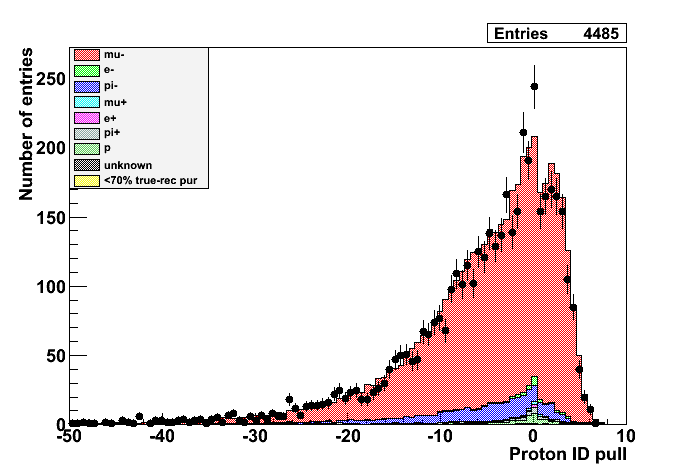
\includegraphics[width=\textwidth]{figures/numu/Cuts/numu/Protpull_run12}
		\caption{$Pull_p$}
	\end{subfigure}
	\begin{subfigure}[t]{0.32\textwidth}
		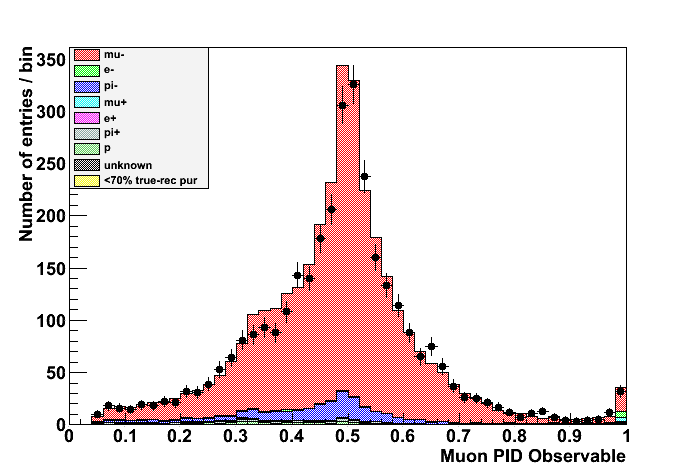
\includegraphics[width=\textwidth]{figures/numu/Cuts/numu/Mulikelihood_run2}
		\caption{$Pull_\mu$}
	\end{subfigure}
	\caption{Pull distributions after selection showing data and MC for \numu analysis}
	\label{fig:numu_pulls}
\end{figure}

The selection criteria then proceeds to split the CC-inclusive sample into the three subsamples: CC$0\pi$, CC$1\pi$ and CCOther. This is based entirely on pion identification in the TPCs and FGDs.

To identify pion candidate(s) a number of cuts are applied:
\begin{itemize}
	\item \textbf{Muon candidate}: The track can not be identified as the above muon candidate.
	
	\item \textbf{Matching beam spill and bunch}: The pion candidate is required to originate from the same beam bunch and spill to the identified muon candidate.
	
	\item \textbf{Track origin}: The pion candidate is required to start in the same FGD fiducial volume as the muon candidate and enter the downstream TPC for PID purposes. The same FGD and TPC track quality and fiducial volume cut is applied for the pion candidate as for the muon candidate.
	
	\item \textbf{Pion PID}: For positive tracks in the TPC, pion, positron and proton hypotheses are tested. For negative tracks, pion and electron hypotheses are tested. 
	
	As for the muon candidate, \autoref{eq:tpc_track_chi2} and \autoref{eq:tpc_track_likelihood} defines the particle likelihoods. For the pion PID, the MIP likelihood in \autoref{eq:tpc_track_mip} is required and in addition a cut on the pion likelihood is invoked,
	\begin{equation}
	\label{tpc_track_pi}
		\mathcal{L}_\pi > 0.3
	\end{equation}
	
	When there is no particle track in the TPC, the FGD PID can be used to count the number of charged pions. However, it can not be used for neutral pions because there is currently no electron or positron reconstruction available. The FGD pion PID proceeds either by:
	\begin{itemize}
		\item \textbf{Michel electron tag}: For low-momentum pion tracks that fail to leave enough hits for track reconstruction, a search for a Michel electron tag is made. It looks for a time-delayed FGD hit cluster out of time with a beam bunch window (so has no associated beam spill or bunch). The number of hits in the delayed time bin should be greater than six for FGD1 and five for FGD2\footnote{Roughly corresponding to 200 photoelectrons, but can't be used as a criteria in FGD2 due to the water layers}. Since no measurement of the track is made, this selection does not give rise to a pion momentum.
		
		\item \textbf{FGD reconstruction}: For higher momentum pions it is required they leave fully contained tracks in the FGD and that the track belongs to the same bunch as the muon candidate. Furthermore, there can only be one pion track reconstructed in the FGD, which eliminates the possibility of a broken track being reconstructed as two pions. The pion candidate is required to be upwards or downwards-going by invoking $|\cos\theta_{\pi,\nu}| > 0.3$, which limits the possibility of traveling along the FGD bars. Finally it is required the pion pull (as a function of track length) $P_\pi$ be $-2 < P_\pi < 2.5$ from simulation studies, shown in \autoref{fig:FGD_pion_pulls}.
	\end{itemize}
\end{itemize}
\begin{figure}[!h]
	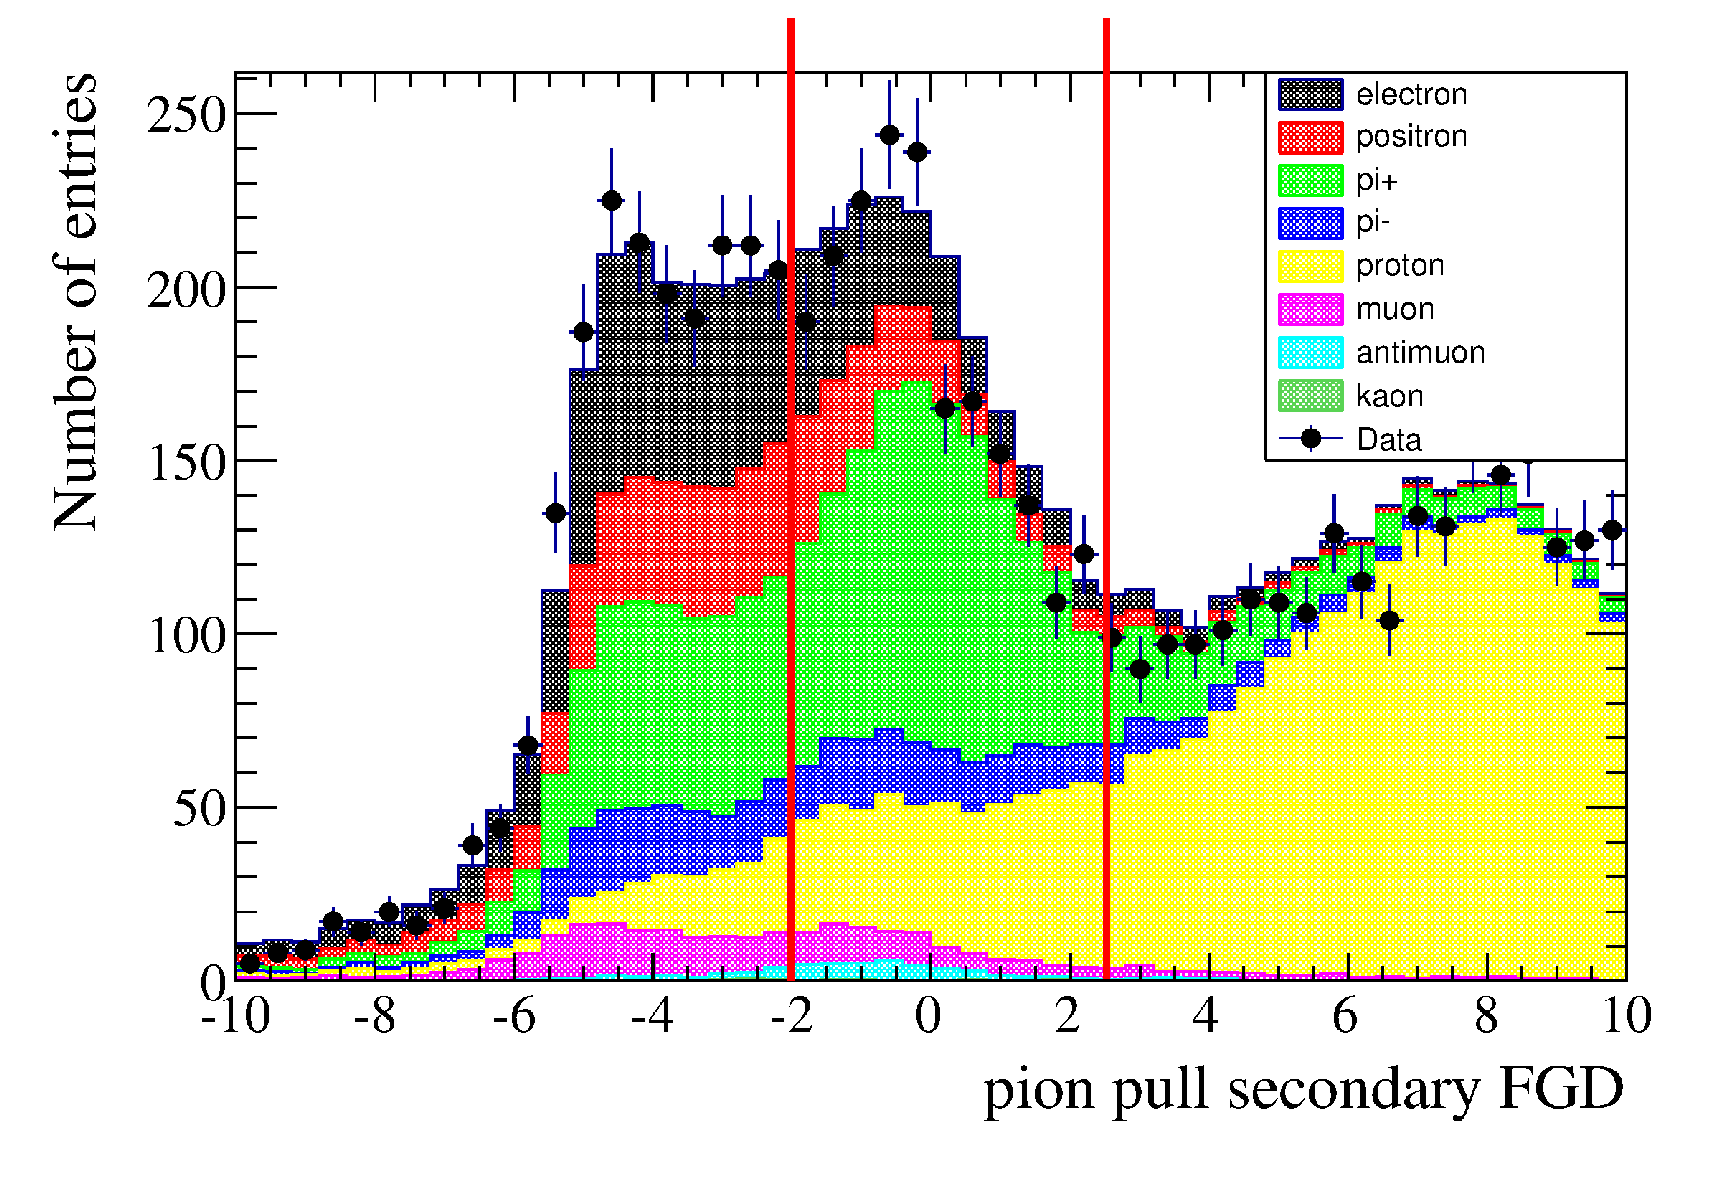
\includegraphics[width=0.5\textwidth]{figures/numu/Cuts/pull_secondarytrack_FGD_all.eps}
	\caption{FGD1 pion pulls for a fully contained track}
	\label{fig:FGD_pion_pulls}
\end{figure}

Then finally the remaining particles can be identified using the TPC PID: 
\begin{itemize}
	\item For a positive particle, it is tagged with type of highest probability. If the most likely particle is a positron but the $p_{reco} > 900\text{ MeV}$ it's tagged as a proton, otherwise a positron
	
	\item For a negative particle, if the probability of a pion is $P_\pi>0.8$ it is tagged as a negative pion, and if not it is assumed an electron
\end{itemize}

Now using information from the TPC PID, FGD Michel electron and FGD PID algorithms the \numu CC-inclusive sample can be categorised into the CC$0\pi$, CC$1\pi$ and CCOther samples:
\begin{itemize}
	\item \textbf{CC0$\pi$}: Contains events with no identified pions, electrons or positrons using the TPC PID. There are no Michel electrons and/or charged pions found in the FGD
	\item \textbf{CC$1\pi$}: Contains events with one reconstructed positively charged pion. The sum of the number of positive pions found in the TPC and the number of Michel electrons is one. If there are no Michel electrons the sum of positive pions in the TPC and fully contained in the FGD is one. If there is a negative pion or electron/positron reconstructed in the TPC it is rejected.
	\item \textbf{CCOther}: All events which are not classified as CC0$\pi$ or CC$1\pi$ fall into this sample. Events with one or more reconstructed negative pions, or neutral pions reconstructed as electron or positron candidates, in the TPC are thereby selected. Event with more than one positive pion based on the TPC and FGD pion counting criteria will also enter into this sample.
\end{itemize}

\paragraph{Efficiency and purity}
Using the aforementioned cuts we can study the lepton tagging efficiency and purity of each ND280 \numu selection. The number of events are the raw number of generated Monte-Carlo events without any weighting applied. We show the efficiencies as a function of reconstructed lepton candidate momentum, $p_{reco}$.

\autoref{fig:cc0pi_topology} shows the topology purity for the CC0$\pi$ selection in FGD1 and FGD2. The purity peak coincides with the event peak with $\sim85\%$ efficiency and falls off in both directions. The true CC$1\pi$ and CCOther topology constitute the selection very similarly, at about $10\%$ across the momentum range. As we move up in momentum the CC DIS cross-sections---the largest contribution to the CCOther final state---increase whilst the CCQE and 2p2h cross-sections---the largest contributions to the CC0$\pi$ final state---decrease. CC1$\pi$ and CC DIS interactions can produce low-momentum pions which aren't reconstructed in the detector and CC DIS can produce a $\pi^-$ which may be mistaken for the lepton candidate \red{show plots of cross-sections?}. Furthermore, the pions can undergo secondary interactions after exiting the nucleus, causing them to be undetected. The NC contribution comes primarily from the NC$1\pi^-$ via resonance interaction, in which the $\pi^-$ is identified as the lepton candidate and there are no other particles in the final state. We also note barely any anti-neutrino contamination, owing to the sign selection from the magnet, the low \numubar flux in FHC and the smaller cross-section. Averaging over the entire range we have purity of $75.5\%$ for FGD1 and $73.5\%$ for FGD2.
\begin{figure}[h]
	\begin{subfigure}[t]{0.49\textwidth}
		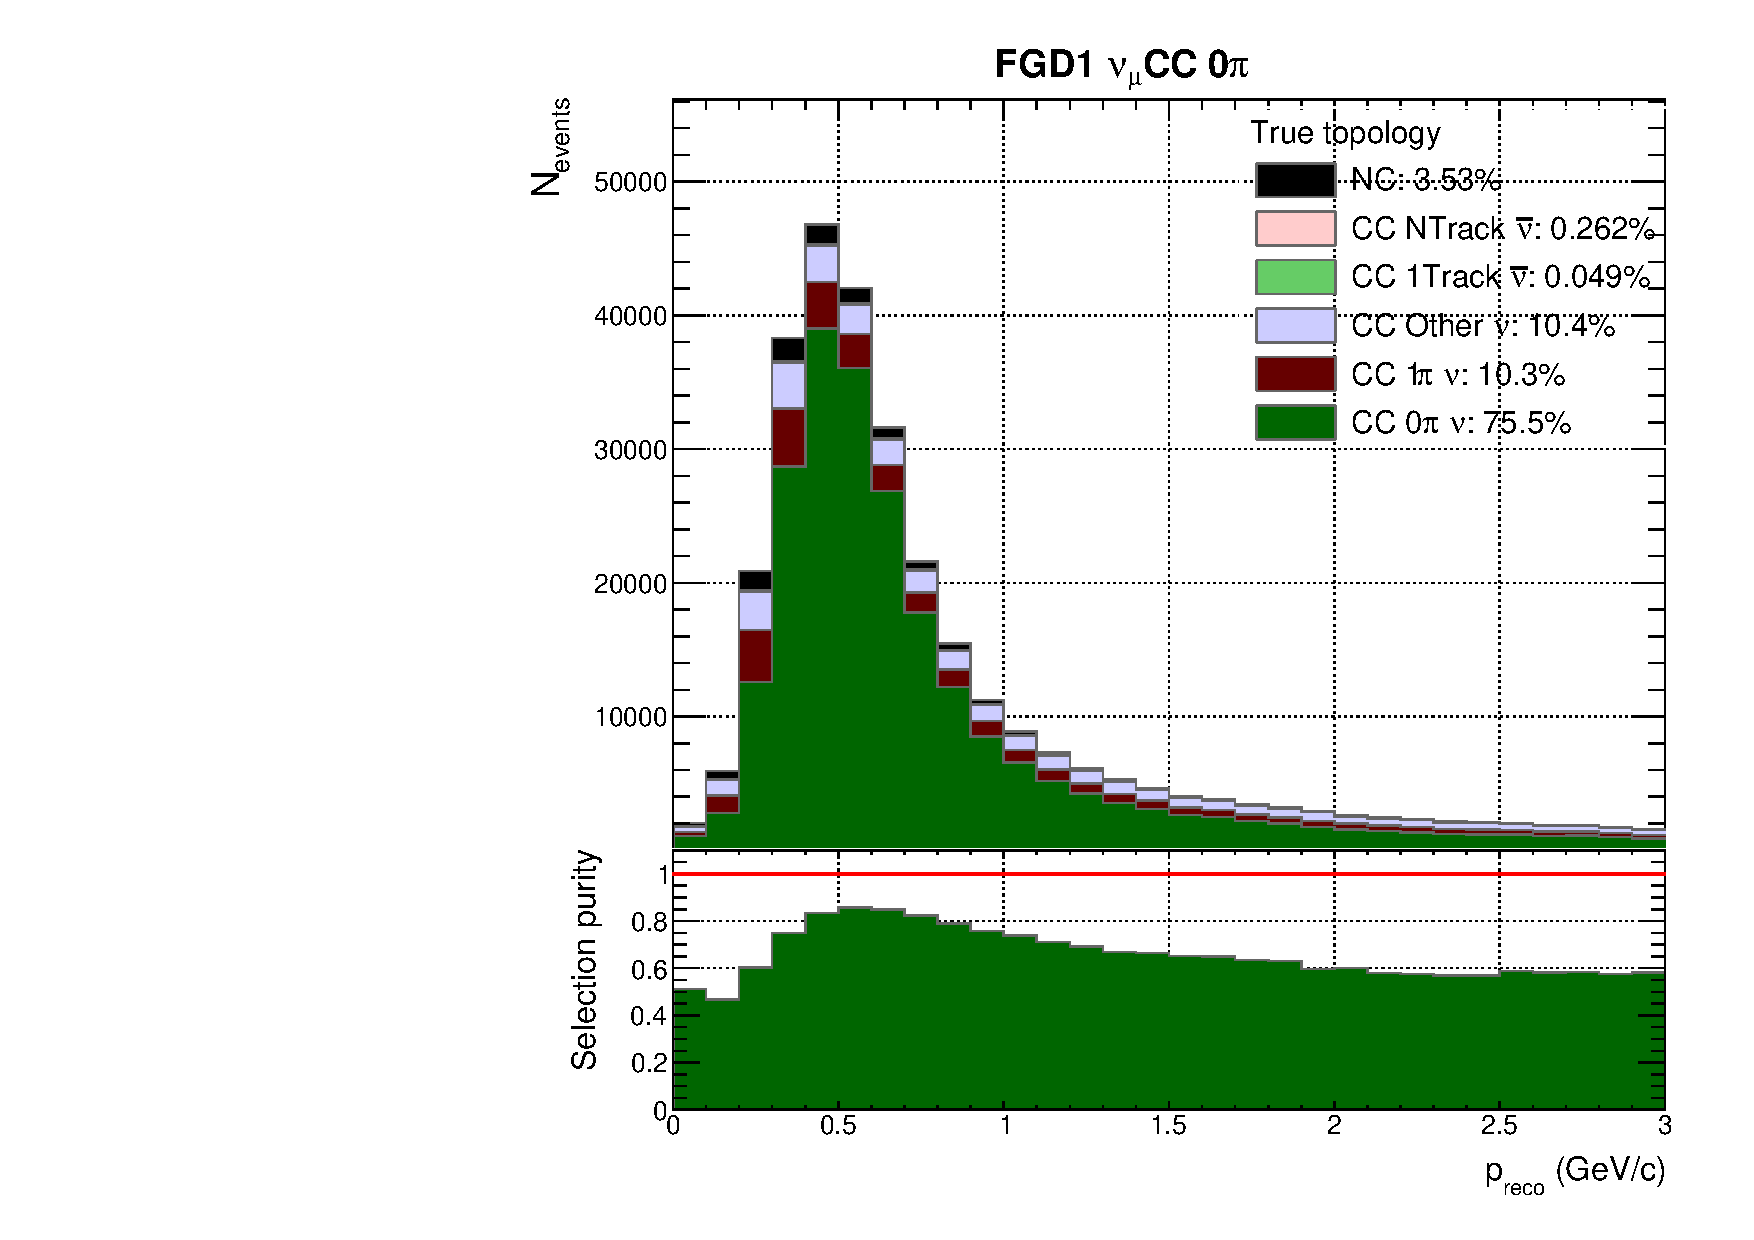
\includegraphics[width=\textwidth,page=1, trim={0mm 0mm 0mm 9mm}, clip]{figures/mach3/selection/2017b_Diag_WithSelection}
		\caption{FGD1}
	\end{subfigure}
	\begin{subfigure}[t]{0.49\textwidth}
		\includegraphics[width=\textwidth,page=7, trim={0mm 0mm 0mm 9mm}, clip]{figures/mach3/selection/2017b_Diag_WithSelection}
		\caption{FGD2}
	\end{subfigure}
	\caption{Breakdown of CC0$\pi$ selection events' true event topology for FGD1 and FGD2 }
	\label{fig:cc0pi_topology}
\end{figure}

\autoref{fig:cc0pi_muon} shows the muon tagging efficiency. We observe good performance over the range of muon momentum, starting with $\sim65\%$ at low momentum, plateauing at $\sim95\%$ above 500 MeV/c for both FGD1 and FGD2, which is where the majority of events reside. Averaging over the entire range, the muon tagging performance is 93.8\% for FGD1 and 93.2\% for FGD2. The largest background is $\pi^-$ from CC$1\pi$, CCOther and NC interactions, in which the $\pi^-$ is either created at the interaction vertex---e.g. an NC$1\pi^-$ via a resonance where there is no $\mu^-$, or a CCOther interaction creating multiple pions in which one $\pi^-$ has a higher reconstructed momentum than the $\mu^-$---or through final-state-interactions (FSI) in which a nucleon, $\pi^0$ or $\pi^+$ undergoes scattering on nucleons in the nucleus to produce the $\pi^-$.
\begin{figure}[!h]
	\begin{subfigure}[t]{0.49\textwidth}
		\includegraphics[width=\textwidth,page=2, trim={0mm 0mm 0mm 9mm}, clip]{figures/mach3/selection/2017b_Diag_WithSelection}
		\caption{FGD1}
	\end{subfigure}
	\begin{subfigure}[t]{0.49\textwidth}
		\includegraphics[width=\textwidth,page=8, trim={0mm 0mm 0mm 9mm}, clip]{figures/mach3/selection/2017b_Diag_WithSelection}
		\caption{FGD2}
	\end{subfigure}
	\caption{Breakdown of selection CC0$\pi$ events' true lepton candidate for FGD1 and FGD2 }
	\label{fig:cc0pi_muon}
\end{figure}

\autoref{fig:cc1pi_topology} shows the topology purity for the CC1$\pi$ selection. Owing to identifying one single $\pi^+$ and one single $\pi^-$, the purity is notably worse for CC1$\pi$ compared to CC0$\pi$ and peaks at $p_{reco}\sim0.4\text{ GeV/c}$ with $\sim70\%$ purity. The purity takes the biggest hit from CCOther feed-down at $25\%$, in which either the lepton candidate is identified as a $\pi^-$ with an accompanying $\pi^+$, or events with a \{$\mu^-$, $\pi^+$, $\pi^{-,0}$\} have the latter pion unreconstructed from high-angle and low momentum tracks, leading to a poorly determined PID. The CCOther feed-down increases with $p_{reco}$ as the CC DIS cross-section increases: the main cause of the decreasing purity with increase $p_{reco}$. The CC0$\pi$ contributions comes from the outgoing proton being reconstructed as a $\pi^+$, or when the nucleon rescatters after exiting the nucleus, producing a pion-like track that gets associated with the primary vertex by mistake. The CC0$\pi$ contribution is concentrated in the first momentum bin, in which it makes up $\sim50\%$. The NC topology contributes 7\% by producing a \{$\pi^-$, $\pi^+$\} state through NC DIS or NC1$\pi$ with FSI which gets reconstructed as the \{$\mu^-$, $\pi^+$\} final state. The purity for CC1$\pi$ across the full momentum range is $58\%$ and very similar for FGD1 and FGD2.
\begin{figure}[!h]
	\begin{subfigure}[t]{0.49\textwidth}
		\includegraphics[width=\textwidth,page=3, trim={0mm 0mm 0mm 9mm}, clip]{figures/mach3/selection/2017b_Diag_WithSelection}
		\caption{FGD1}
	\end{subfigure}
	\begin{subfigure}[t]{0.49\textwidth}
		\includegraphics[width=\textwidth,page=9, trim={0mm 0mm 0mm 9mm}, clip]{figures/mach3/selection/2017b_Diag_WithSelection}
		\caption{FGD2}
	\end{subfigure}
	\caption{Breakdown of selection CC1$\pi$ events' true event topology for FGD1 and FGD2 }
	\label{fig:cc1pi_topology}
\end{figure}

\autoref{fig:cc1pi_muon} shows the muon tagging efficiency for CC1$\pi^+$. As for the purity, the efficiency is comparably worse due to the additional pion requirement, averaging at 83\% across the $p_{reco}$ range. Common with the CC0$\pi$ efficiency in \autoref{fig:cc0pi_muon} the major background is $\pi^-$, which now constitutes 11\% instead of 4\%. The $\pi^-$ comes primarily from DIS interactions and CC1$\pi^0$ via resonances in which the $\pi^0$ undergoes a charge-exchange FSI, as discussed earlier. The $\pi^+$ contribution comes from high momentum pions which do not bend sufficiently to get a good PID: since the initial CC-inclusive search is done based on highest-momentum track this track is selected as the lepton candidate which curves similarly to a high-momentum $\mu^-$. As $p_{reco}$ increases the efficiency tends to similar values as the CC0$\pi$ selection.
\begin{figure}[!h]
	\begin{subfigure}[t]{0.49\textwidth}
		\includegraphics[width=\textwidth,page=4, trim={0mm 0mm 0mm 9mm}, clip]{figures/mach3/selection/2017b_Diag_WithSelection}
		\caption{FGD1}
	\end{subfigure}
	\begin{subfigure}[t]{0.49\textwidth}
		\includegraphics[width=\textwidth,page=10, trim={0mm 0mm 0mm 9mm}, clip]{figures/mach3/selection/2017b_Diag_WithSelection}
		\caption{FGD2}
	\end{subfigure}
	\caption{Breakdown of selection CC1$\pi$ events' true lepton candidate for FGD1 and FGD2 }
	\label{fig:cc1pi_muon}
\end{figure}

\red{Add part looking at how the pion is tagged and number of events}

\red{Show plots for \cosmu?}

\autoref{fig:ccoth_topology} shows the topology purity for the CCOther selection. As expected from the other purities, CCOther increases with $p_{reco}$ due to the increase in the CC DIS cross-section. The CC0$\pi$ and CC1$\pi$ topology seeps in to this selection by creating $\pi^{\pm,0}$ after exiting the nucleus that become(s) wrongly associated with the primary interaction vertex, or by the reconstruction falsely identifying an outgoing proton as a $\pi^+$. In the NC case, it is enough to have a interaction which produces a \{$\pi^-, \pi^0$\} combination, which can happen directly through NC DIS or indirectly with NC$1\pi$ via resonances, in which a secondary interaction occurs and the new track gets wrongly associated to the primary vertex. Initially, the purity starts at 35-40\% and plateaus around 80\% at $p_{reco} \sim 1.5\text{ GeV/c}$. Overall, the purity of the selection is 65\% for both FGDs over the entire range, with $\sim10\%$ each from NC, CC0$\pi$ and CC1$\pi$.
\begin{figure}[!h]
	\begin{subfigure}[t]{0.49\textwidth}
		\includegraphics[width=\textwidth,page=5, trim={0mm 0mm 0mm 9mm}, clip]{figures/mach3/selection/2017b_Diag_WithSelection}
		\caption{FGD1}
	\end{subfigure}
	\begin{subfigure}[t]{0.49\textwidth}
		\includegraphics[width=\textwidth,page=11, trim={0mm 0mm 0mm 9mm}, clip]{figures/mach3/selection/2017b_Diag_WithSelection}
		\caption{FGD2}
	\end{subfigure}
	\caption{Breakdown of selection CCOther events' true event topology for FGD1 and FGD2 }
	\label{fig:ccoth_topology}
\end{figure}

\autoref{fig:ccoth_muon} shows the muon tag efficiency for the CC Other sample, which is notably worse than for previous selections: on average 73\%. This is expected, since the CCOther selection has at least 2 tracks (1$\mu^-$, 1$\pi^{\pm}$, 1$\pi^0$) but often even more. It is sufficient to have an interaction in which $N_\pi \ge 2$ and $p_{\pi} > p_{\mu}$ to wrongly identify the lepton candidate. Owing to the many tracks in this topology due to the CC and NC DIS interaction, it is no surprise to see a 20\% contribution from $\pi^-$. Furthermore, at low $p_{reco}$ electrons are selected a majority of the time, coming from two sources: 1) relatively high threshold of \numu CC DIS compared to \nue CC DIS due to the muon mass (even though the \nue flux is much lower than \numu \red{show this}) and 2) since the CCOther topology is the only topology to allow for $\pi^0$, these are likely to produce $e^\pm$ pairs in the TPC. If the $\pi^0$ shower occurs early in the TPC and the interaction vertex is traced to a downstream layer of the FGD, the electron may be falsely associated with the interaction vertex, and if $p_e > p_\mu$ is picked as the highest momentum candidate. To pass the TPC $\mu$ PID cut we would require a low momentum $e^-$ to match the dE/dx of a $\mu^-$, which in \autoref{fig:TPC_dedx} happens at $p\sim100\text{ MeV/c}$.
\begin{figure}[h]
	\begin{subfigure}[t]{0.49\textwidth}
		\includegraphics[width=\textwidth,page=6, trim={0mm 0mm 0mm 9mm}, clip]{figures/mach3/selection/2017b_Diag_WithSelection}
		\caption{FGD1}
	\end{subfigure}
	\begin{subfigure}[t]{0.49\textwidth}
		\includegraphics[width=\textwidth,page=12, trim={0mm 0mm 0mm 9mm}, clip]{figures/mach3/selection/2017b_Diag_WithSelection}
		\caption{FGD2}
	\end{subfigure}
	\caption{Breakdown of selection CCOther events' true lepton candidate for FGD1 and FGD2 }
	\label{fig:ccoth_muon}
\end{figure}

\subsection{Event selection cuts, \numubar in RHC}
\label{sec:numubar_sel}
The anti-neutrino selections CC1Track and CCNTrack have the same event quality and fiducial volume cut as the neutrino selection, and the muon candidate track is required to pass through the TPC downstream of the struck FGD. However, its highest momentum track is required to be the highest momentum positive track for its muon PID (a $\mu^+$ coming from a \numubar interaction). Furthermore, it has a larger background of ``wrong-sign'' events: \numu interactions producing $\mu^-$, but also \numu interactions producing $\pi^+$ which may be identified as the lepton candidate.\red{SHOW PLOT OF THIS, e.g. numubar flux with numu background in there} Hence, the selection cuts proceed marginally differently:
\begin{itemize}
	\item \textbf{Positive multiplicity}: The muon candidate track charge is required to be a highest momentum positive track, which removes a large amount of \numu background interactions
	
	\item \textbf{TPC veto}: Veto backwards-going events starting in the FGD and events coming from the P0D and the magnet by utilising the upstream TPCs. If the upstream TPC of an FGD has hits the event is rejected
	
	\item \textbf{Positive muon identification}: The TPC PID outlined for the \numu selections are used to select the positive muon candidate, with the cuts optimised for $\mu^+$. 
	
	$\mathcal{L}_{MIP}$ is defined identically to \autoref{eq:tpc_track_mip} although the cut is now placed at 0.9, and still applies only to particles with $p < 500\text{ MeV}$. The muon likelihood $\mathcal{L}_\mu$ is also modified to $0.1 < \mathcal{L}_\mu < 0.7$ which removes protons and positive pions from the \numu background. The upper bound at 0.7 is present to reject low energy wrong-sign muons ($\mu^-$), which are misidentified as positive tracks. The likelihood distributions and impact of these cuts are shown in \autoref{fig:numubar_likelihood} and \autoref{fig:numubar_likelihood_sel} for the selected lepton candidate. \autoref{fig:numubar_pulls} shows the TPC PID pulls for run5+6. \red{REMEMBER THAT THIS IS NOT PRESENT FOR PSYCHE V3}
\end{itemize}

\begin{figure}[!h]
	\begin{subfigure}[t]{0.49\textwidth}
		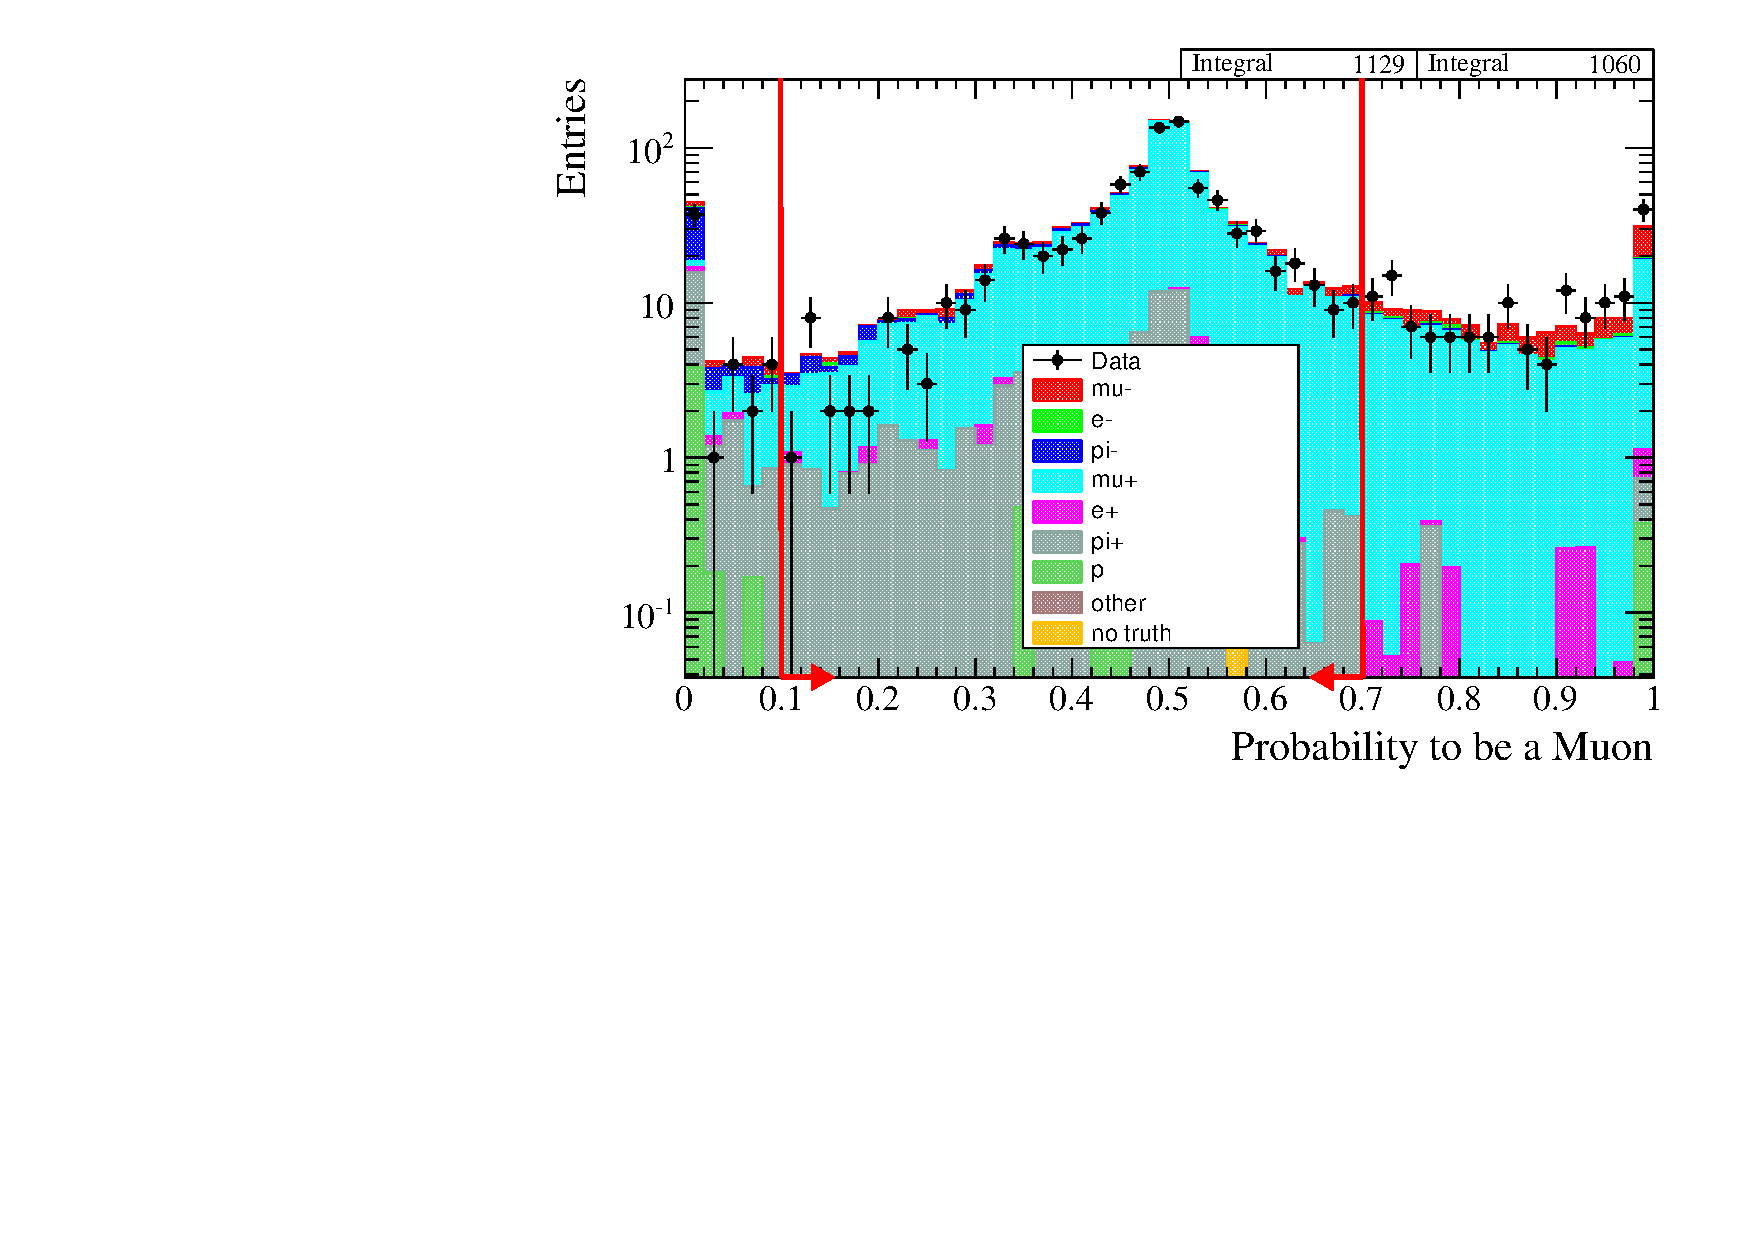
\includegraphics[width=\textwidth]{figures/numu/Cuts/numubar/likemu_numubar}
		\caption{$\mathcal{L}_\mu$}
	\end{subfigure}
	\begin{subfigure}[t]{0.49\textwidth}
		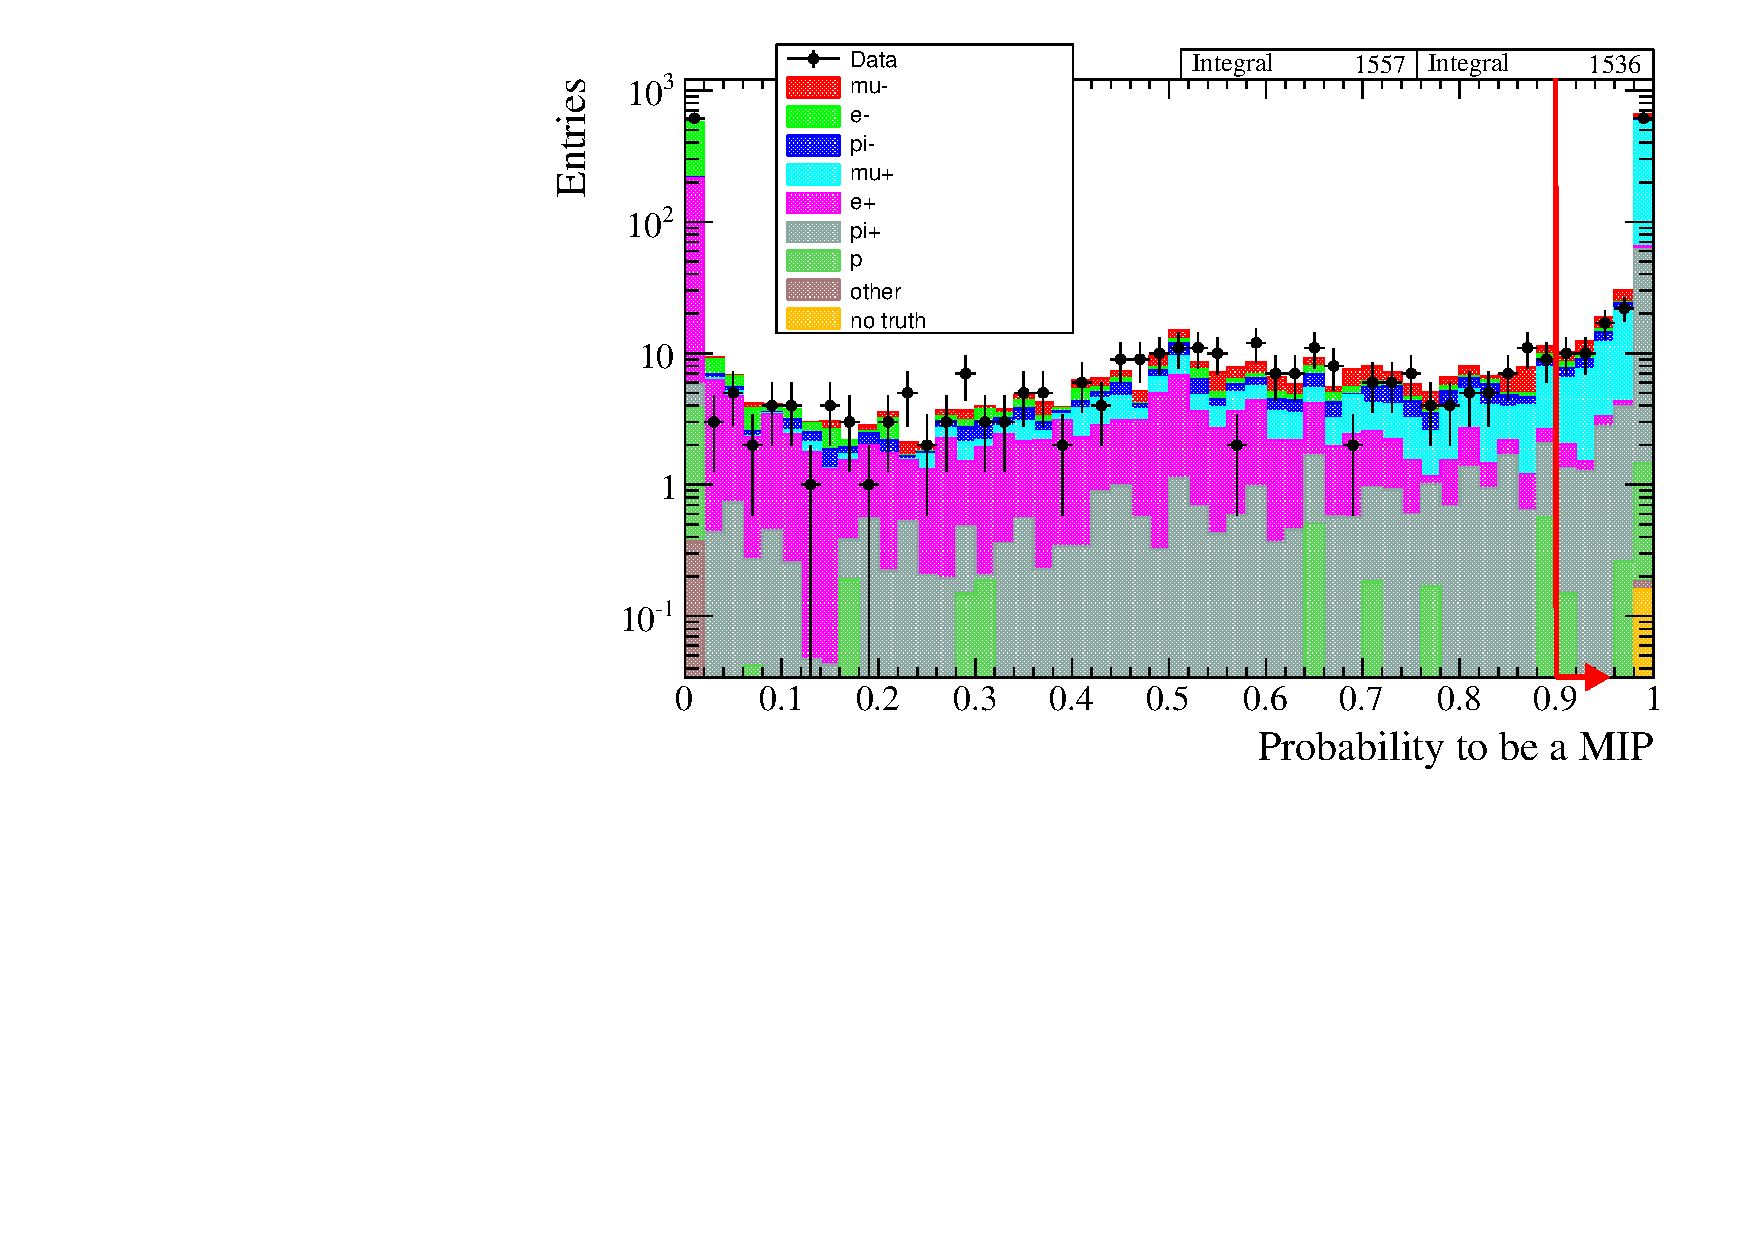
\includegraphics[width=\textwidth]{figures/numu/Cuts/numubar/likemip_numubar}
		\caption{$\mathcal{L}_{MIP}$}
	\end{subfigure}
	\caption{Likelihood distributions for $\mu$ and MIP using run5+6 \numubar data, used in \numubar RHC selections}
	\label{fig:numubar_likelihood}
\end{figure}

\begin{figure}[!h]
	\begin{subfigure}[t]{0.49\textwidth}
		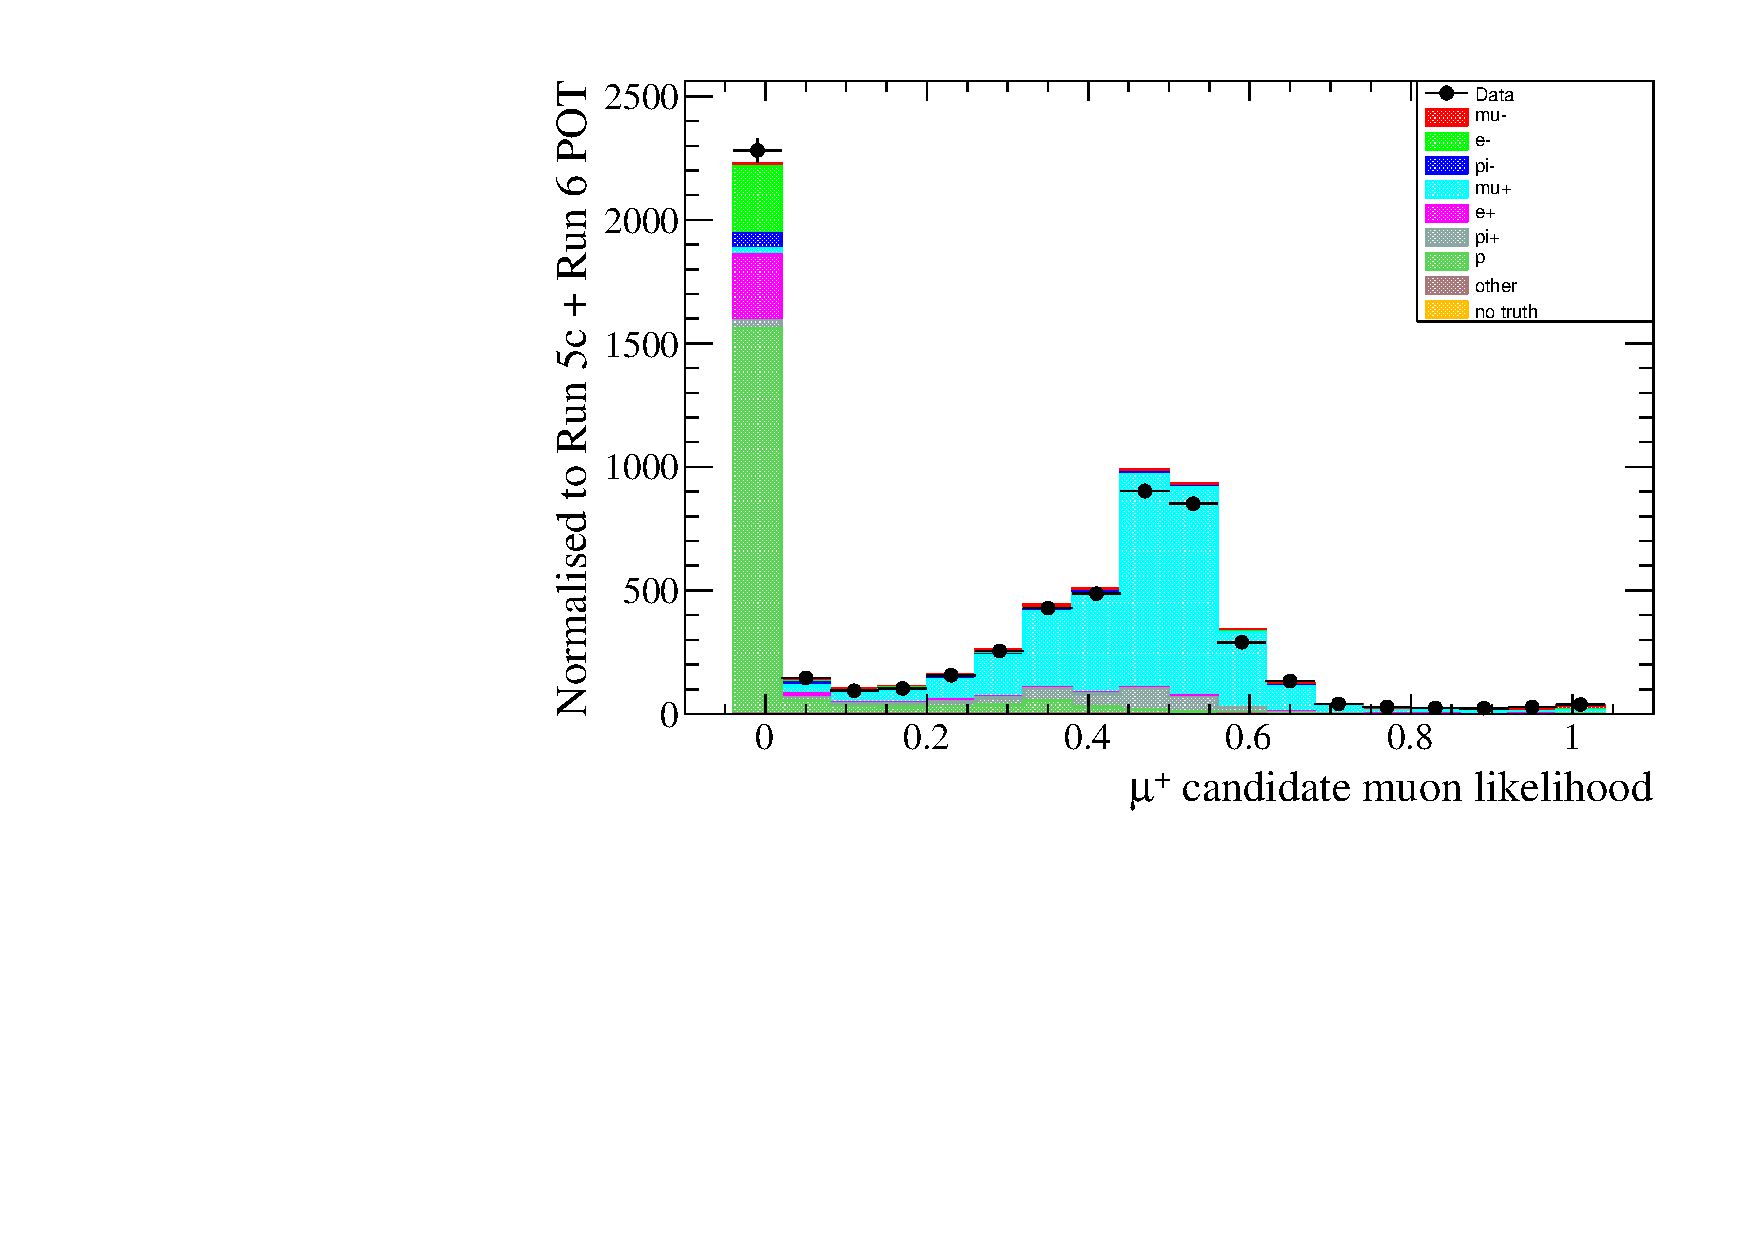
\includegraphics[width=\textwidth]{figures/numu/Cuts/numubar/selmu_likemu_particle}
		\caption{$\mathcal{L}_\mu$}
	\end{subfigure}
	\begin{subfigure}[t]{0.49\textwidth}
		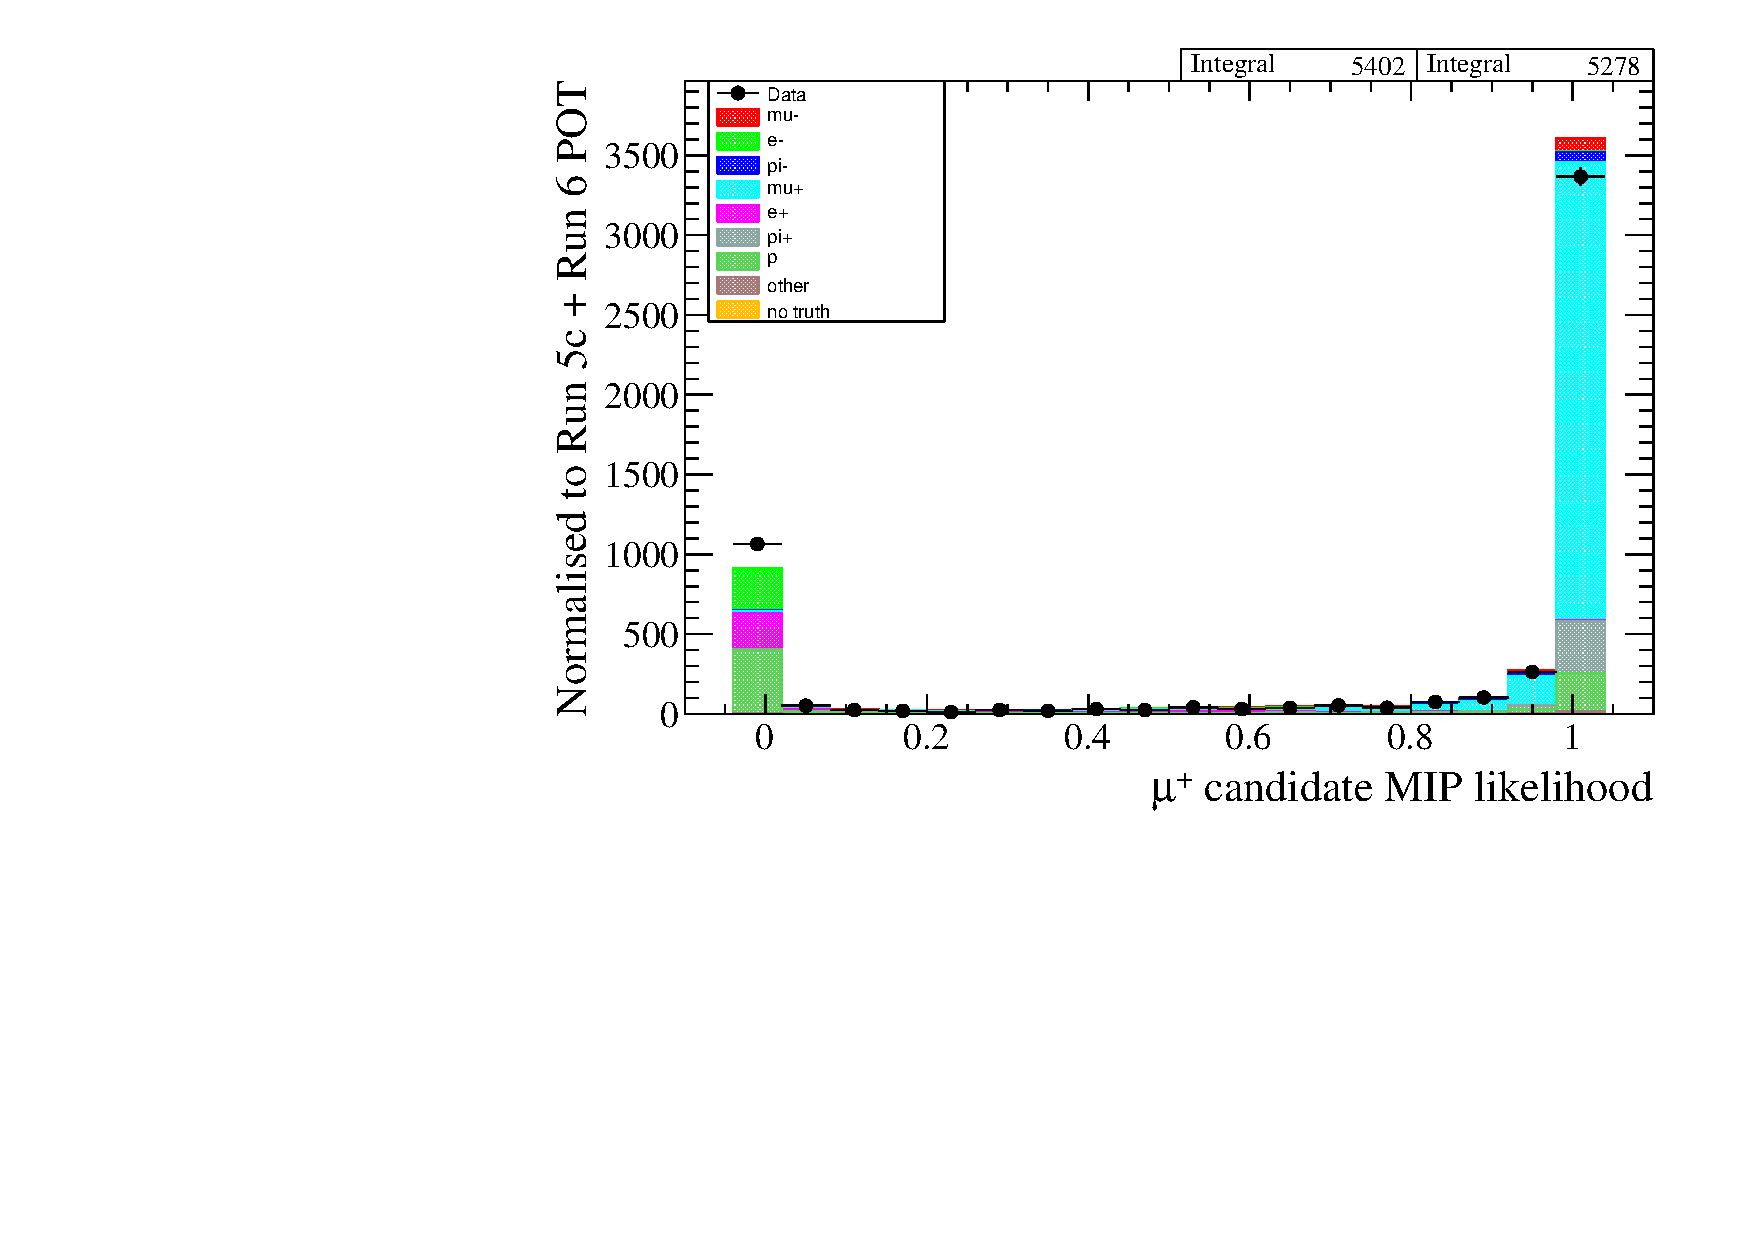
\includegraphics[width=\textwidth]{figures/numu/Cuts/numubar/selmu_likemip_particle}
		\caption{$\mathcal{L}_{MIP}$}
	\end{subfigure}
	\caption{Likelihood distributions for the selected lepton candidate using run5+6 \numubar data, used in \numubar RHC selections}
	\label{fig:numubar_likelihood_sel}
\end{figure}

\begin{figure}[!h]
	\begin{subfigure}[t]{0.32\textwidth}
		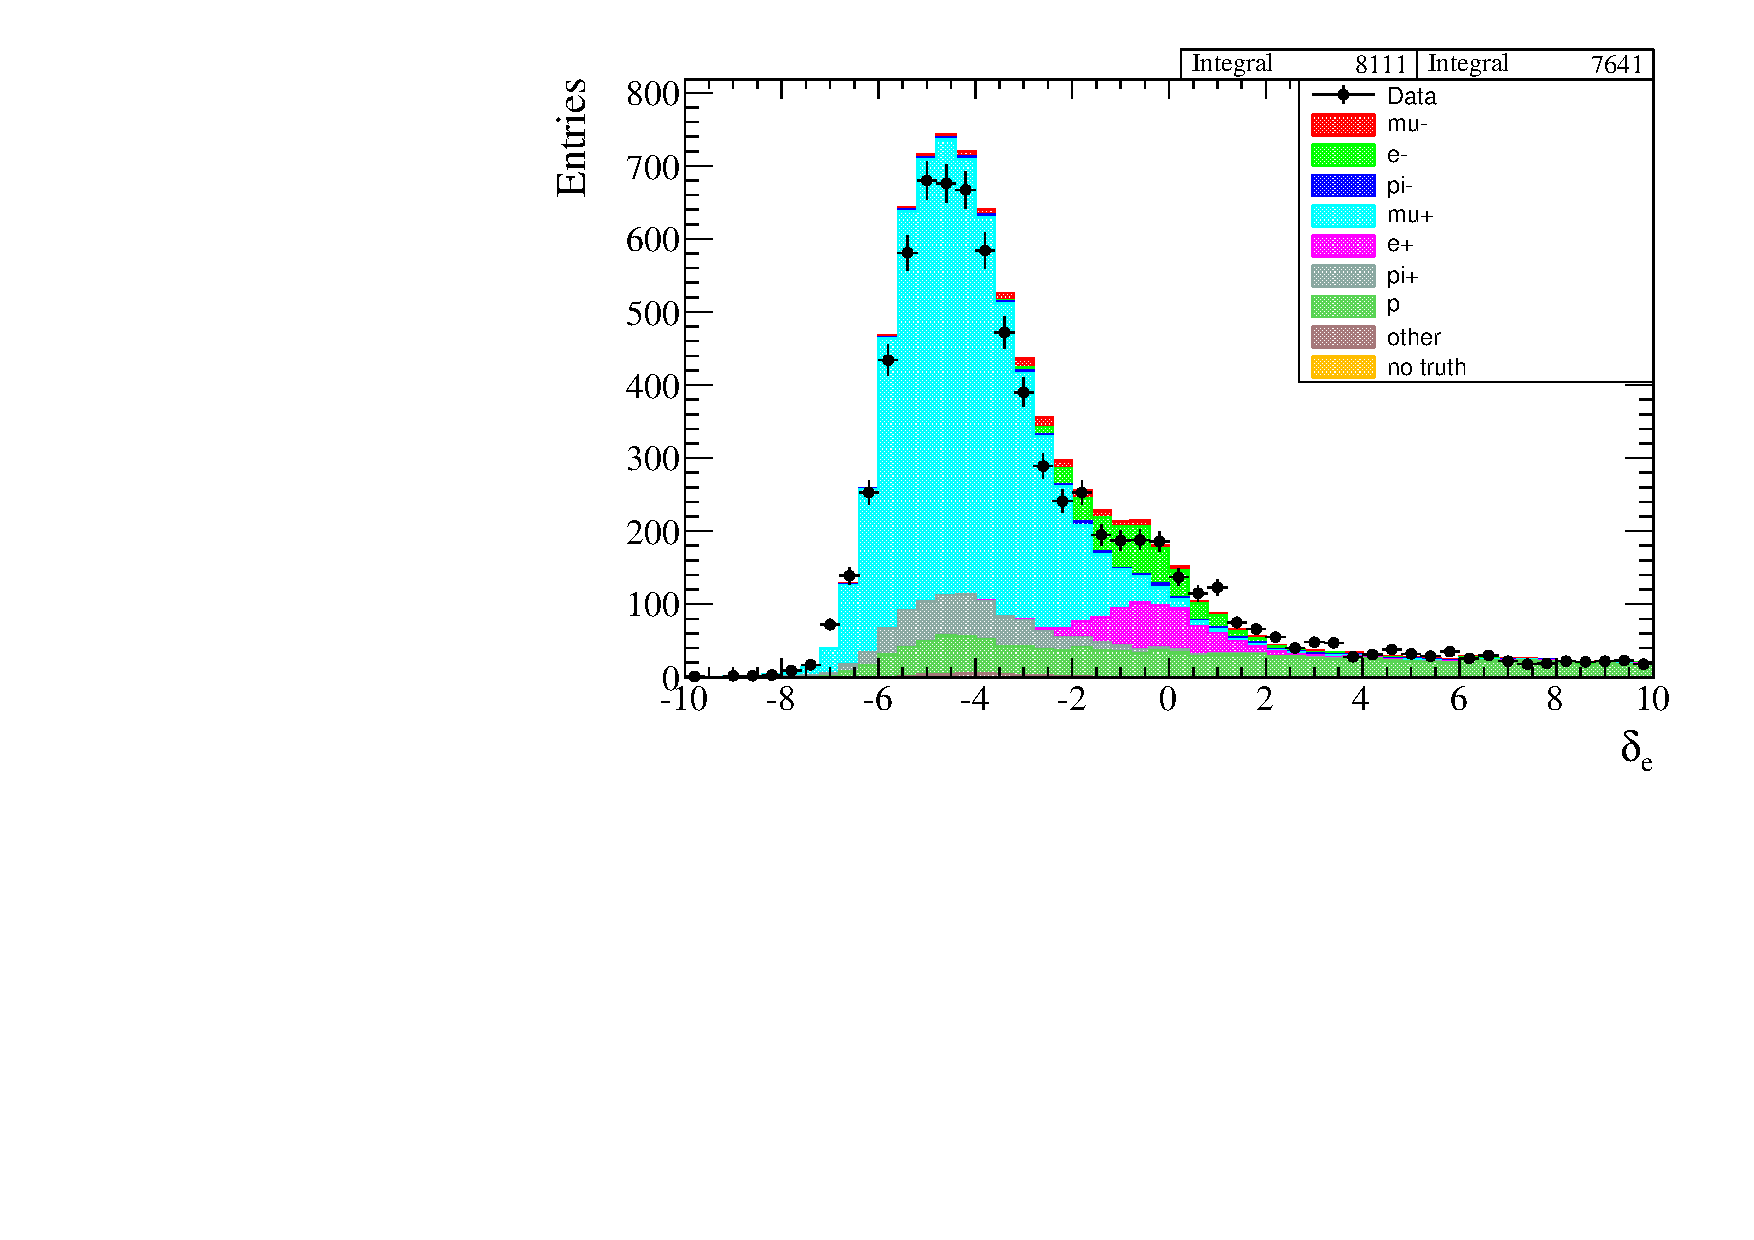
\includegraphics[width=\textwidth]{figures/numu/Cuts/numubar/presel_pullele_part}
		\caption{$Pull_e$}
	\end{subfigure}
	\begin{subfigure}[t]{0.32\textwidth}
		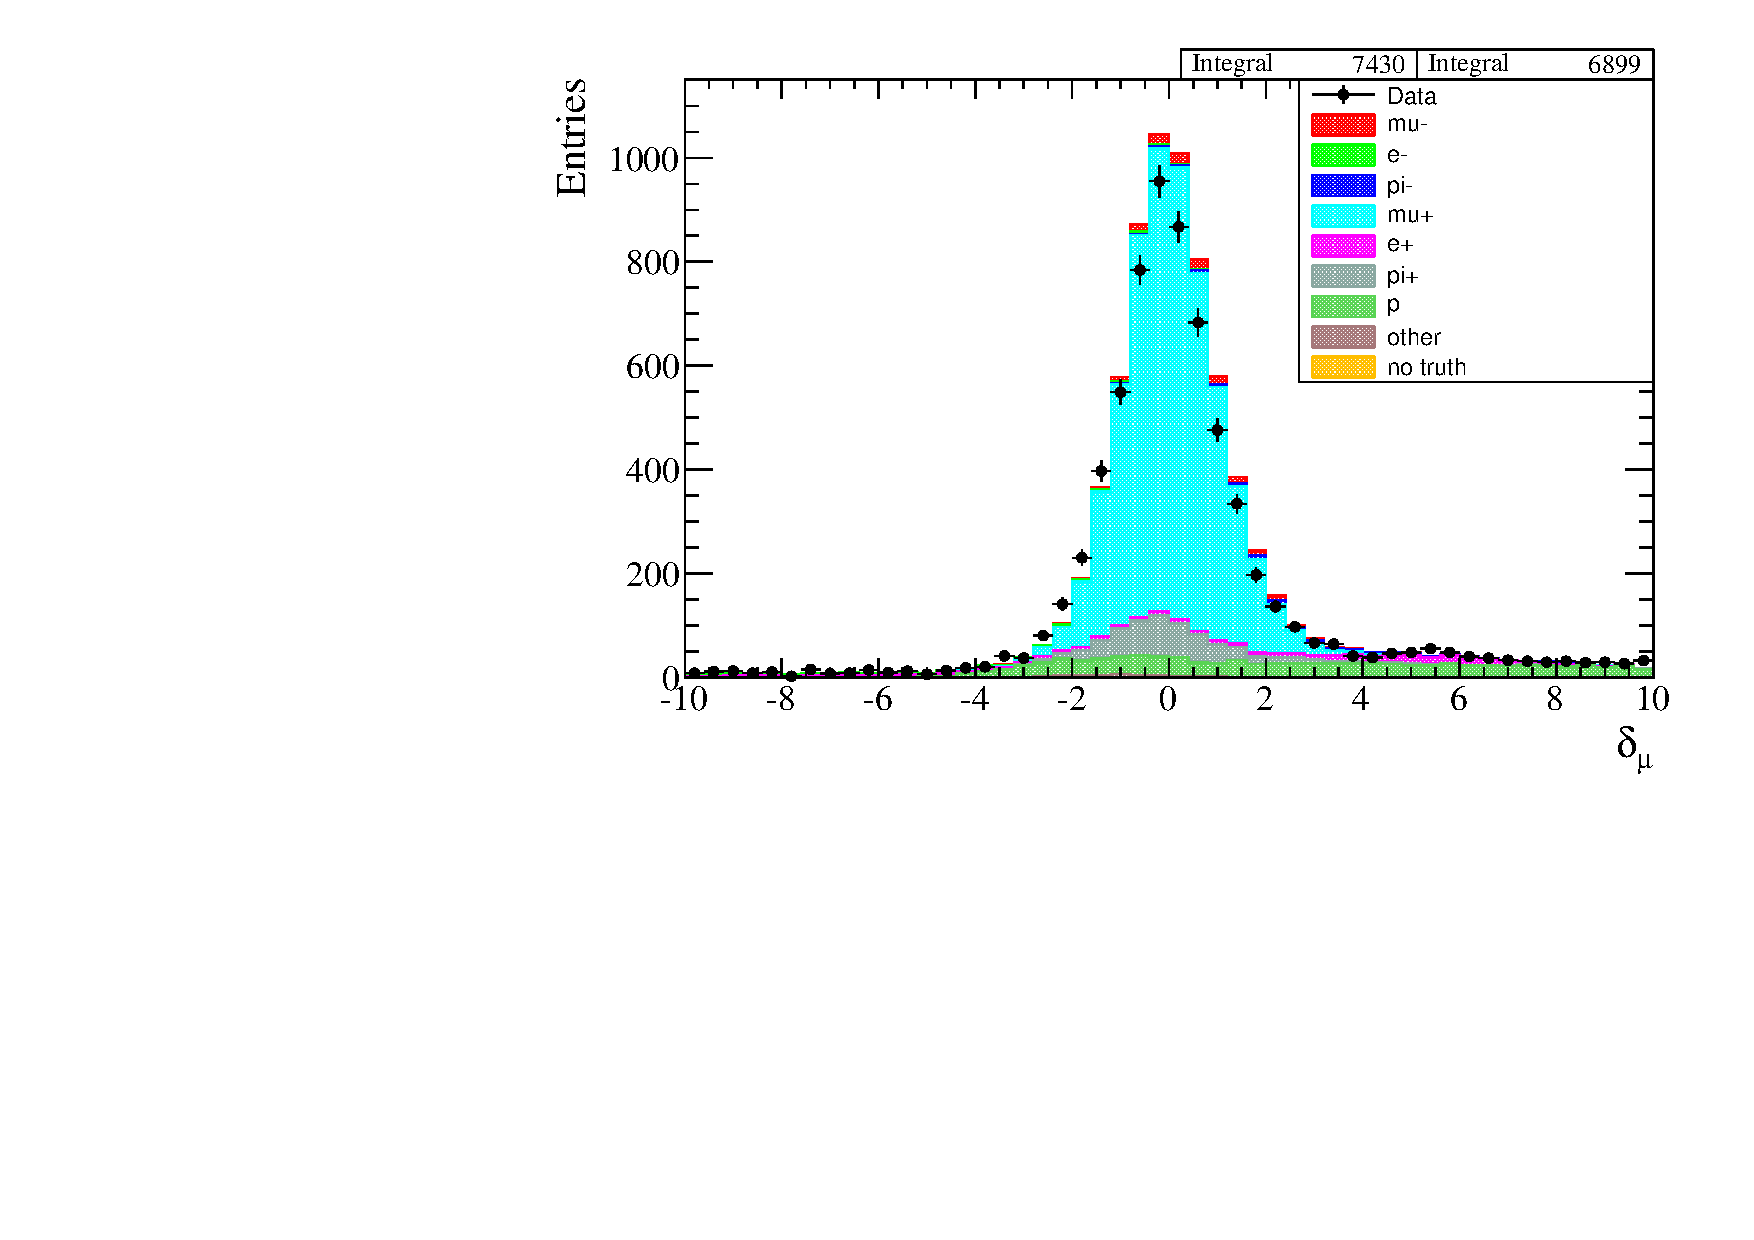
\includegraphics[width=\textwidth]{figures/numu/Cuts/numubar/presel_pullmu_part}
		\caption{$Pull_\mu$}
	\end{subfigure}
	\begin{subfigure}[t]{0.32\textwidth}
		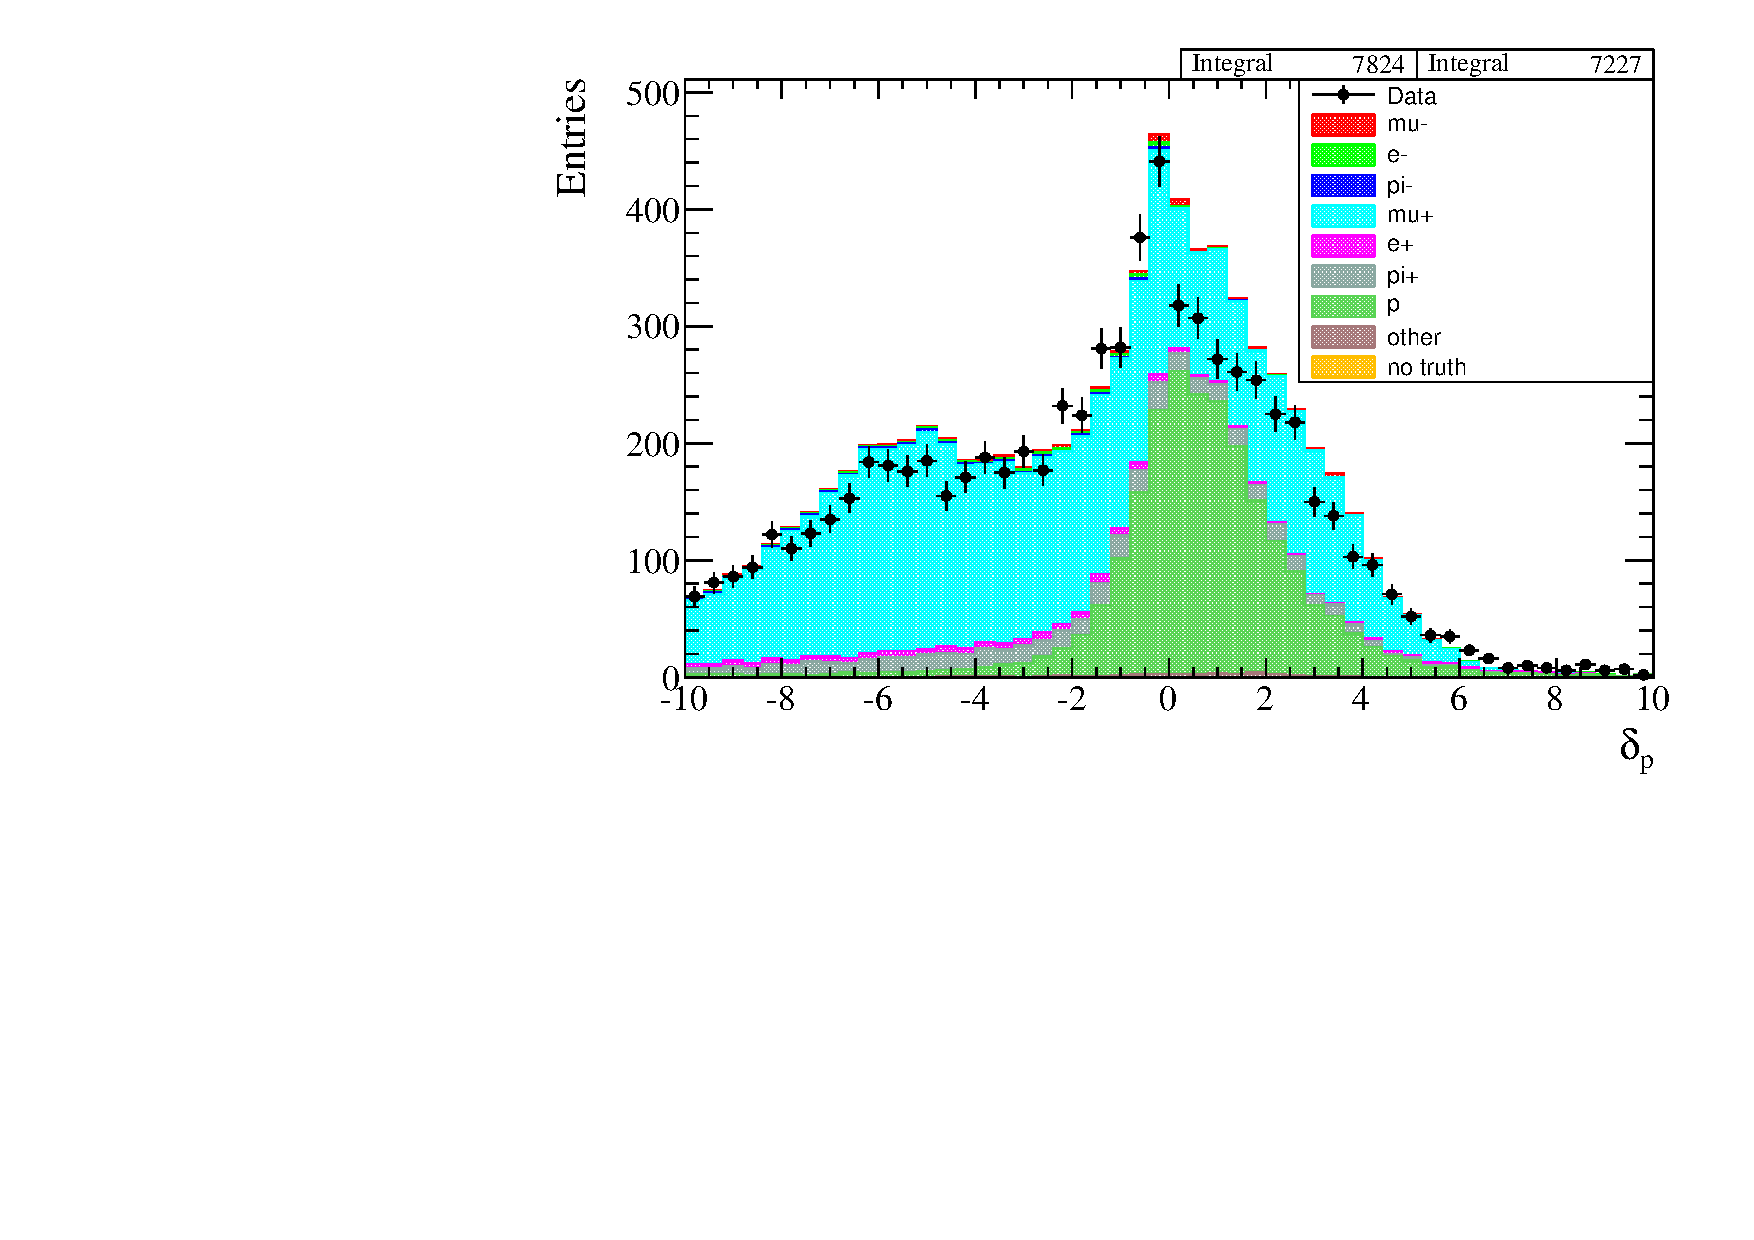
\includegraphics[width=\textwidth]{figures/numu/Cuts/numubar/presel_pullp_part}
		\caption{$Pull_p$}
	\end{subfigure}
	\caption{Pulls used in the TPC PID used in \numubar RHC selections}
	\label{fig:numubar_pulls}
\end{figure}

Once the \numubar CC-inclusive selection is run the aforementioned pion reconstruction is applied. The \numubar CC1Track selection has one positive muon and does not have any charged or neutral pions in the final state. Importantly, the \numubar CC1Track selection has a higher efficiency in selecting the muon candidate than the \numu CC0$\pi$ selection due to the \numubar resonant interactions producing a $\pi^-$, not a $\pi^+$, which are promptly absorbed in the nucleus and so do not leave a track to be (falsely) identified as a muon candidate. The \numubar CCNTrack selection contains the remaining particles passing the \numubar CC-inclusive selection, containing at least one neutral or charged pion and/or any number of heavier mesons.

\paragraph{Efficiency and purity}
As for the \numu case, we study the efficiency and purities of the anti-neutrino CC1Track and CCNTrack samples.

\autoref{fig:ccnubar1trk_topology} shows the \numubar CC 1 track topology purity. The purity peaks at 85\% with the event distribution peak ($p_{reco}\sim 0.6\text{ GeV}$) and decreases to $\sim60\%$ at higher momentum. The wrong-sign \numu equivalent selection have a small effect, notable only at low momentum. The largest background is the \numubar N tracks topology, in which one of the pions are unreconstructed. The NC topology enters primarily by the NC1$\pi^+$ via resonance interaction, in which the $\pi^+$ is reconstructed as a $\mu^+$. Over the whole range the purity is 76.7\% where the analogous \numu selection in \autoref{fig:cc0pi_topology} had a purity of 75.5\%, so are very similar in performance.
\begin{figure}[h]
	\begin{subfigure}[t]{0.49\textwidth}
		\includegraphics[width=\textwidth,page=13, trim={0mm 0mm 0mm 9mm}, clip]{figures/mach3/selection/2017b_Diag_WithSelection}
		\caption{FGD1}
	\end{subfigure}
	\begin{subfigure}[t]{0.49\textwidth}
		\includegraphics[width=\textwidth,page=17, trim={0mm 0mm 0mm 9mm}, clip]{figures/mach3/selection/2017b_Diag_WithSelection}
		\caption{FGD2}
	\end{subfigure}
	\caption{Breakdown of \numubar CC 1Trk selection events' true event topology for FGD1 and FGD2 }
	\label{fig:ccnubar1trk_topology}
\end{figure}

\autoref{fig:ccnubar1trk_muon} shows the muon efficiency for \numubar CC 1 track selection. As with the \numu selections, both FGDs have efficiencies of 90\% over the whole range, peaking at 95\% at the event distribution maximum around $p_{reco} \sim 0.5\text{ GeV/c}$. The wrong-sign (\numubar) background makes up 1\% of selected lepton candidates, and NC 5\%.
\begin{figure}[h]
	\begin{subfigure}[t]{0.49\textwidth}
		\includegraphics[width=\textwidth,page=14, trim={0mm 0mm 0mm 9mm}, clip]{figures/mach3/selection/2017b_Diag_WithSelection}
		\caption{FGD1}
	\end{subfigure}
	\begin{subfigure}[t]{0.49\textwidth}
		\includegraphics[width=\textwidth,page=18, trim={0mm 0mm 0mm 9mm}, clip]{figures/mach3/selection/2017b_Diag_WithSelection}
		\caption{FGD2}
	\end{subfigure}
	\caption{Breakdown of \numubar CC 1Trk selection events' true lepton candidate for FGD1 and FGD2 }
	\label{fig:ccnubar1trk_muon}
\end{figure}

As with the \numu samples, the CCNTrack selection purity in \autoref{fig:ccnubarNtrk_topology} is much lower than for the 1 track. It peaks at 60\% and decreases to 40\% at intermediate $p_{reco}$ to increase to 60\% at higher momentum. Overall, the wrong-sign CC N track topology (\numu) is the largest contribution at 27\%, the NC contribution is 14\% and \numubar CC 1 track is non-negligable at 12\% for both FGDs. Since the CCNtrack selection only requires $N>1$, the \numu CC N track enters by the \{$\mu^-$,$\pi^+$\} being identified as \{$\pi^-$, $\mu^+$\}, on top of the usual possibilities of broken tracks and missed secondary pions. The CC1Track contamination comes from energetic protons being reconstructed as a $\mu^+$ or $\pi^+$, and lesser so producing secondary pions and/or nucleons, leading to more particles associated with the primary vertex.
\begin{figure}[!h]
	\begin{subfigure}[t]{0.49\textwidth}
		\includegraphics[width=\textwidth,page=15, trim={0mm 0mm 0mm 9mm}, clip]{figures/mach3/selection/2017b_Diag_WithSelection}
		\caption{FGD1}
	\end{subfigure}
	\begin{subfigure}[t]{0.49\textwidth}
		\includegraphics[width=\textwidth,page=19, trim={0mm 0mm 0mm 9mm}, clip]{figures/mach3/selection/2017b_Diag_WithSelection}
		\caption{FGD2}
	\end{subfigure}
	\caption{Breakdown of \numubar CC NTrk selection events' true event topology for FGD1 and FGD2 }
	\label{fig:ccnubarNtrk_topology}
\end{figure}

\autoref{fig:ccnubarNtrk_muon} shows the selected lepton candidate, which over the entire momentum range is 54\%. At low momentum the efficiency is very poor but peaks at $p_{reco} \sim 0.5 \text{ GeV/c}$ at about 60\%. $\pi^+$ make up $\sim24\%$ of the lepton candidates, having the largest impact between 0.5-1.5 GeV/c. At $\sim 1.5\text{ GeV/c}$ the ``Other'' category rises sharply, making up 30\% of the lepton candidates. This population is predominantly protons being identified as $\mu^+$ in the TPC PID algorithm due to the dE/dx, which happens when $1.3 < p < 1.7 \text{ GeV/c}$ as seen in \autoref{fig:TPC_dedx}. Looking ahead at the \numu in RHC muon efficiency in \autoref{fig:ccnubarnuNtrk_muon}, the ``Other'' population contributes a mere 0.6\% over the entire momentum range since the lepton candidate is required to be of negative charge. After the proton ``bump'' the efficiency rises to 60\% again.
\begin{figure}[!h]
	\begin{subfigure}[t]{0.49\textwidth}
		\includegraphics[width=\textwidth,page=16, trim={0mm 0mm 0mm 9mm}, clip]{figures/mach3/selection/2017b_Diag_WithSelection}
		\caption{FGD1}
	\end{subfigure}
	\begin{subfigure}[t]{0.49\textwidth}
		\includegraphics[width=\textwidth,page=20, trim={0mm 0mm 0mm 9mm}, clip]{figures/mach3/selection/2017b_Diag_WithSelection}
		\caption{FGD2}
	\end{subfigure}
	\caption{Breakdown of \numubar CC NTrk selection events' true lepton candidate for FGD1 and FGD2 }
	\label{fig:ccnubarNtrk_muon}
\end{figure}

\subsection{Event selection, \numu in RHC}
\label{sec:numu_in_nubar_sel}
In anti-neutrino mode there is a large fraction of \numu interactions, owing partly to the larger \numu cross-section and partly due to the higher flux background. \red{show plots of this}. The same pre-selection cuts apply for the \numu in RHC selection as for the previous selections presented in \autoref{sec:numu_sel} and \autoref{sec:numubar_sel}.

The CC-inclusive selection proceeds by:
\begin{itemize}
	\item \textbf{Negative multiplicity}: The highest momentum track is required to be the highest momentum negative track, which starts the seeding track. The $\mu^-$ identification uses the TPC PID on the highest momentum negative track. 
	
	\item \textbf{TPC PID}: The PID proceeds by the MIP requirement in \autoref{eq:tpc_track_mip} for particles with $p_\mu < 500 \text{ MeV/c}$, accepting candidate tracks with $\mathcal{L}_{MIP} > 0.7$.
	
	Similar to \autoref{sec:numubar_sel}, a lower and upper bound is set $0.1 < \mathcal{L}_\mu < 0.8$, which rejects protons and mis-reconstructed $\mu^+$. The effect of these cuts can be seen in \autoref{fig:nu_numubar_likelihood}.
\end{itemize}

\begin{figure}[!h]
	\begin{subfigure}[t]{0.49\textwidth}
		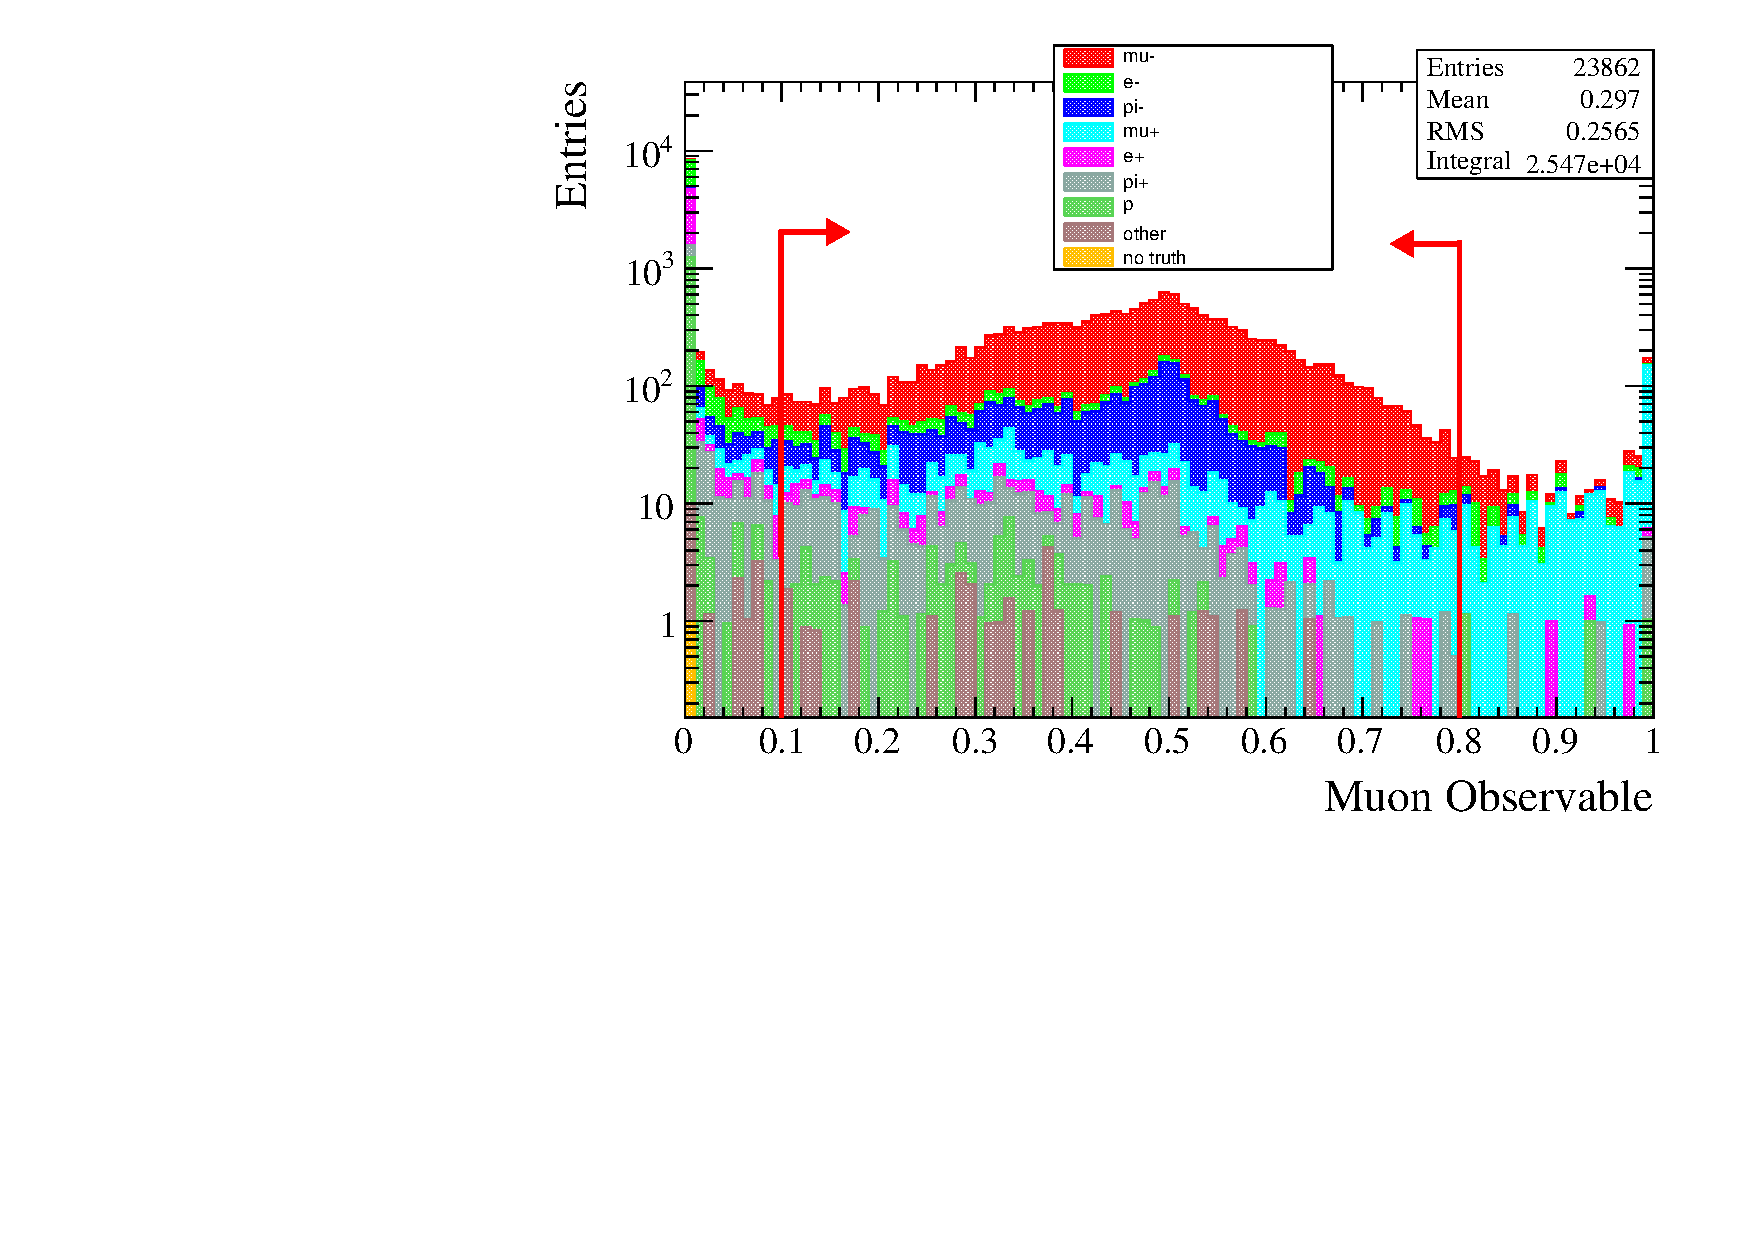
\includegraphics[width=\textwidth]{figures/numu/Cuts/numu_in_numubar/MuonLikelihood_prod6B_NuMuCont_FGD1Only}
		\caption{$\mathcal{L}_\mu$}
	\end{subfigure}
	\begin{subfigure}[t]{0.49\textwidth}
		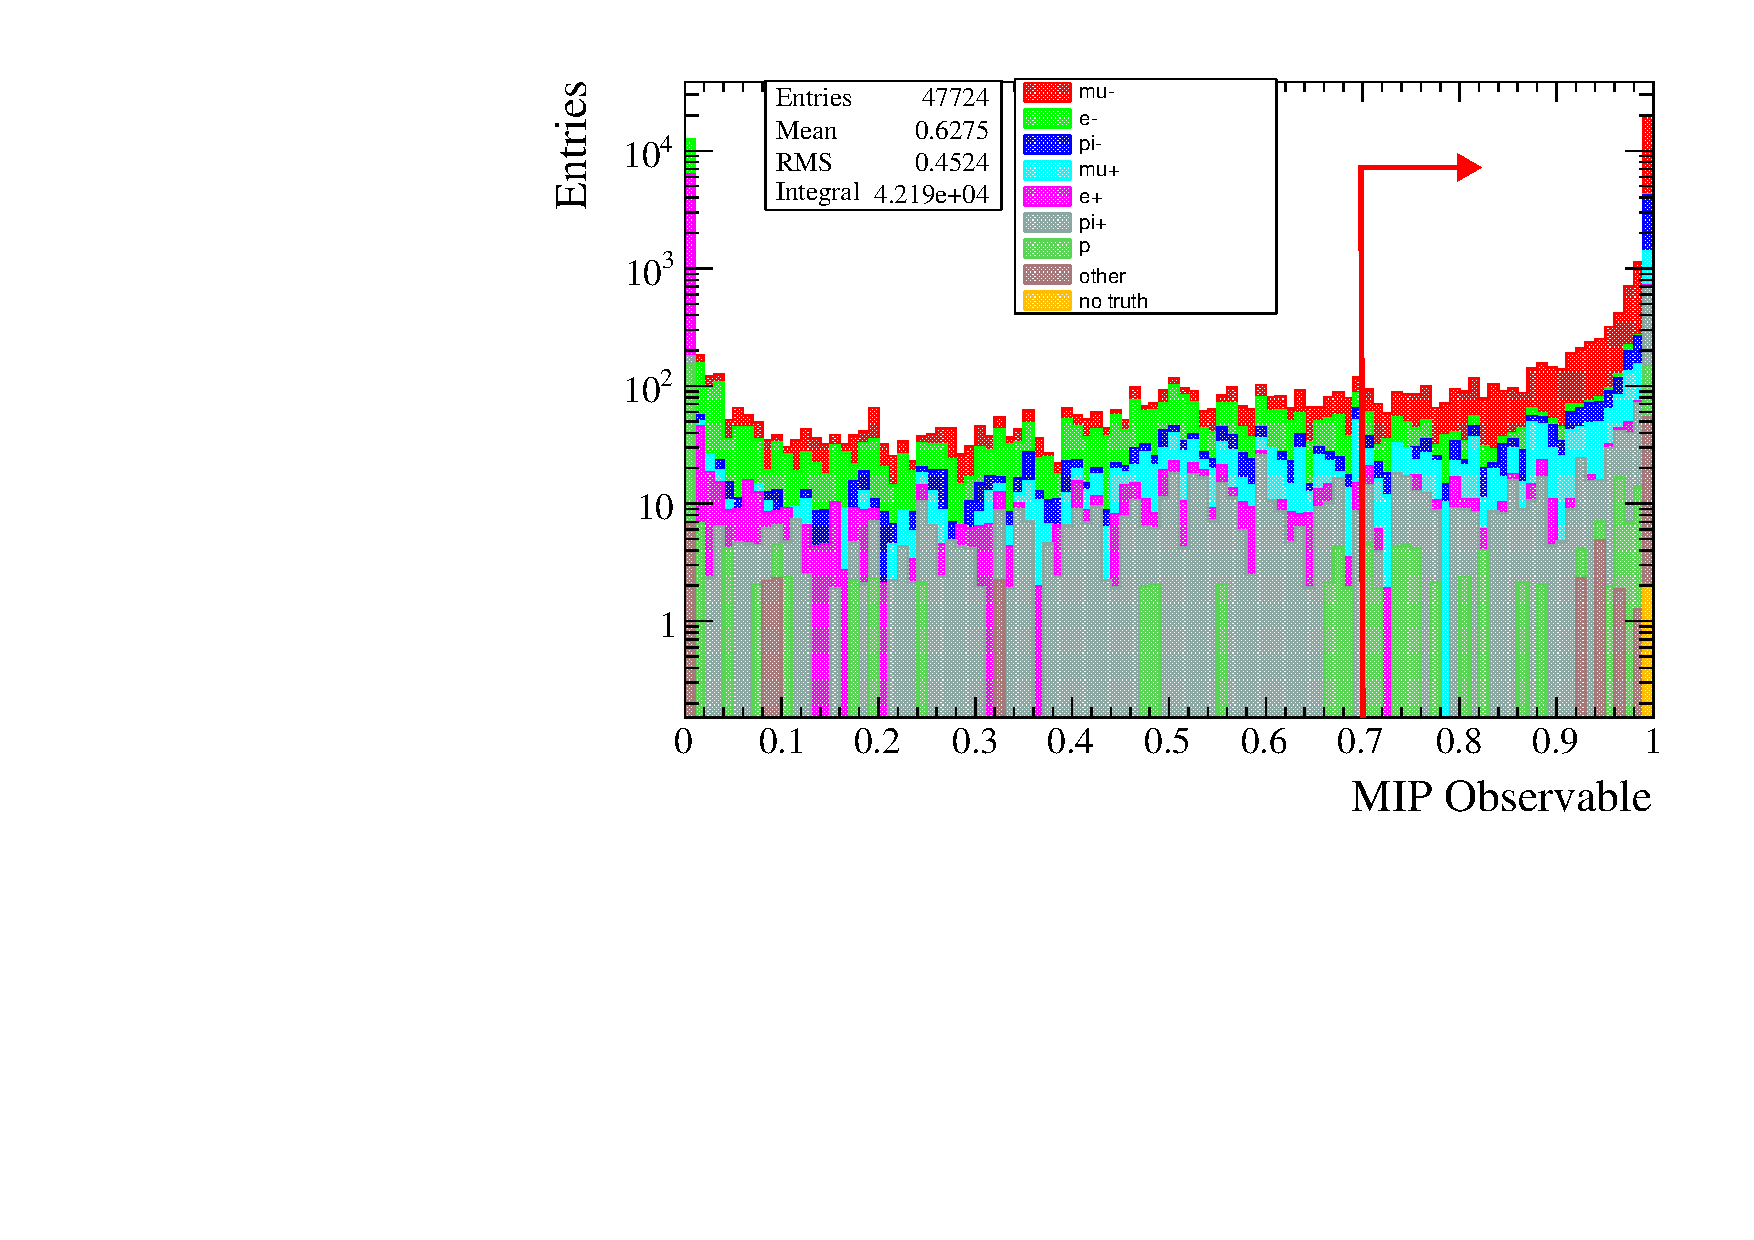
\includegraphics[width=\textwidth]{figures/numu/Cuts/numu_in_numubar/MipLikelihood_LogScale}
		\caption{$\mathcal{L}_{MIP}$}
	\end{subfigure}
	\caption{Likelihood distributions for $\mu$ and MIP using run5+6 \numubar data, used in \numu in RHC selections}
	\label{fig:nu_numubar_likelihood}
\end{figure}

The \numu in RHC selection then breaks down the CC-inclusive selection into CC1Track and CCNTrack, based entirely on the number of TPC-FGD matched tracks. Events with one such reconstructed track enters the CC1Track selection, and events with any other number of tracks regardless of PID, enter the CCNTrack selection. Hence the \numu RHC selection is analogous to the \numubar RHC selection.

\paragraph{Efficiency and purity}
As in previous sections we now study the muon tagging efficiency and topological purity of the final \numu in RHC selections.

\autoref{fig:ccnubarnu1trk_topology} shows the purity of the CC1Track selection, where we note a poor purity at low momentum, plateauing at 60\% at 0.8 GeV/c, averaging at 52\%. The overall \numu CCNtrack contribution is 29\%, 10 percentage units larger than for \numubar and is roughly constant over the full range. The wrong-sign contribution is 10\% in total, and NC is 10\%. The wrong-sign and NC contributions happen primarily at low momentum and vanish above $p_{reco}=1\text{ GeV/c}$.
\begin{figure}[!h]
	\begin{subfigure}[t]{0.49\textwidth}
		\includegraphics[width=\textwidth,page=21, trim={0mm 0mm 0mm 9mm}, clip]{figures/mach3/selection/2017b_Diag_WithSelection}
		\caption{FGD1}
	\end{subfigure}
	\begin{subfigure}[t]{0.49\textwidth}
		\includegraphics[width=\textwidth,page=25, trim={0mm 0mm 0mm 9mm}, clip]{figures/mach3/selection/2017b_Diag_WithSelection}
		\caption{FGD2}
	\end{subfigure}
	\caption{Breakdown of \numu in RHC CC 1Trk selection events' true event topology for FGD1 and FGD2 }
	\label{fig:ccnubarnu1trk_topology}
\end{figure}

\autoref{fig:ccnubarnu1trk_muon} shows the muon efficiency which closely follows the pattern of the purity. The efficiency is very poor up until 300 MeV/c and then sharply rises to plateau at 95\% at 1 GeV/c. However the event distribution peaks in region of low efficiency, causing the average to be 75\%. The background varies significantly in the low momentum range: at lowest momentum it's composed of $e^\pm$ since the TPC has similar energy loss for $e$ and $\mu$ in this region. Around the event peak, 1/2-2/3 of the selected leptons are background, almost equally wrong-sign muons and both signs of pions. The $\pi^-$ background comes primarily from NC1$\pi^-$ and \numubar CC1$\pi^-$ where the muon is missed.
\begin{figure}[!h]
	\begin{subfigure}[t]{0.49\textwidth}
		\includegraphics[width=\textwidth,page=22, trim={0mm 0mm 0mm 9mm}, clip]{figures/mach3/selection/2017b_Diag_WithSelection}
		\caption{FGD1}
	\end{subfigure}
	\begin{subfigure}[t]{0.49\textwidth}
		\includegraphics[width=\textwidth,page=26, trim={0mm 0mm 0mm 9mm}, clip]{figures/mach3/selection/2017b_Diag_WithSelection}
		\caption{FGD2}
	\end{subfigure}
	\caption{Breakdown of \numu in RHC CC 1Trk selection events' true lepton candidate for FGD1 and FGD2 }
	\label{fig:ccnubarnu1trk_muon}
\end{figure}

For the NTrack distribution purity in \autoref{fig:ccnubarnuNtrk_topology} we approximately 60\% purity, which plateaus at 70\% above 1.5 GeV/c. The largest background is from same-sign CC1Trk where a broken track or secondary interaction creates a false second (or more) track associated with the vertex. The NC contribution is approximately same size and shape to the wrong-sign CCNTrk, at 10\%, largest below $p_{reco}\sim 1\text{ GeV/c}$. For NC the contribution comes from reconstructing a \{$\pi^-$,$\pi^{0,+}$\} pair as a \{$\mu^-$, $\pi^{0,+}$\} pair, and the wrong sign NTrack comes from \{$\mu^+$, $\pi^-$\} as \{$\pi^+$, $\mu^-$\}, just as in the \numubar RHC selection, for which the NC contamination was 14\% and wrong-sign NTrack was 27\%. However, the \numubar RHC CCNtrack selection additionally stands the risk of a proton being reconstructed as the $\mu^+$, which is why the purity is worse.
\begin{figure}[!h]
	\begin{subfigure}[t]{0.49\textwidth}
		\includegraphics[width=\textwidth,page=23, trim={0mm 0mm 0mm 9mm}, clip]{figures/mach3/selection/2017b_Diag_WithSelection}
		\caption{FGD1}
	\end{subfigure}
	\begin{subfigure}[t]{0.49\textwidth}
		\includegraphics[width=\textwidth,page=27, trim={0mm 0mm 0mm 9mm}, clip]{figures/mach3/selection/2017b_Diag_WithSelection}
		\caption{FGD2}
	\end{subfigure}
	\caption{Breakdown of \numu in RHC CC NTrk selection events' true event topology for FGD1 and FGD2 }
	\label{fig:ccnubarnuNtrk_topology}
\end{figure}

Inspecting the muon tagging efficiency in \autoref{fig:ccnubarnuNtrk_muon}, we observe several traits common with the \numubar CCNTrack and \numu CCOther selections: at low momentum the lepton tag is primarily from $e^-$ due to the similar energy loss of $e$, $\mu$ and $\pi$ in this region; as we increase lepton candidate momentum we create $\mu$,$\pi$ systems in which the $\pi^-$ has the higher momentum and is assumed the $\mu^-$ candidate. The efficiency rises sharply at 0.3 GeV/c and plateaus at 80\% above 1 GeV/c, coinciding with the event distribution peak. Over the entire range the efficiency is 74\% and the $\pi^-$ background is 20\%.
\begin{figure}[!h]
	\begin{subfigure}[t]{0.49\textwidth}
		\includegraphics[width=\textwidth,page=24, trim={0mm 0mm 0mm 9mm}, clip]{figures/mach3/selection/2017b_Diag_WithSelection}
		\caption{FGD1}
	\end{subfigure}
	\begin{subfigure}[t]{0.49\textwidth}
		\includegraphics[width=\textwidth,page=28, trim={0mm 0mm 0mm 9mm}, clip]{figures/mach3/selection/2017b_Diag_WithSelection}
		\caption{FGD2}
	\end{subfigure}
	\caption{Breakdown of \numu in RHC CC NTrk selection events' true lepton candidate for FGD1 and FGD2 }
	\label{fig:ccnubarnuNtrk_muon}
\end{figure}

A summary of all selections' efficiency and purities is shown in \autoref{tab:eff_pur_summary}.
\begin{table}[!h]
	\centering
	\begin{tabular}{ l | c c }
		\hline
		\hline
		Selection 					   & Efficiency (\%) & Purity (\%) \\ 
		\hline
		\FGDCCNoPi{1}{\numu}           & 93.8  & 75.5  \\% \hline
		\FGDCCNoPi{2}{\numu}           & 93.2  & 73.5  \\% \hline
		\hline
		\FGDCCOnePi{1}{\numu}          & 83.3  & 58.0  \\% \hline
		\FGDCCOnePi{2}{\numu}          & 83.1  & 57.1  \\% \hline
		\hline
		\FGDCCOther{1}{\numu}          & 73.0  & 65.3  \\% \hline
		\FGDCCOther{2}{\numu}          & 73.4  & 64.9  \\% \hline
		\hline
		\FGDCCOneTrk{1}{\numubar}      & 90.0  & 76.7  \\% \hline
		\FGDCCOneTrk{2}{\numubar}      & 89.6  & 76.7  \\% \hline
		\hline
		\FGDCCNTrk{1}{\numubar}   	   & 54.1  & 45.1  \\% \hline
		\FGDCCNTrk{2}{\numubar}        & 53.8  & 43.9  \\% \hline
		\hline
		\FGDCCOneTrk{1}{\numu} in RHC  & 76.5  & 52.2  \\% \hline
		\FGDCCOneTrk{2}{\numu} in RHC  & 74.9  & 51.8  \\% \hline
		\hline
		\FGDCCNTrk{1}{\numu} in RHC    & 73.9  & 60.9  \\% \hline
		\FGDCCNTrk{2}{\numu} in RHC    & 74.2  & 61.4  \\% \hline
		\hline
		\hline
	\end{tabular}
	\caption{Efficiency and purity summary for all selections with the range $0 < p_{reco} < 3\text{ GeV/c}$}
	\label{tab:eff_pur_summary}
\end{table}

\section{Binning}
We expect largely similar kinematics across the two FGDs so apply the same binning in reconstructed muon momentum, \pmu, and cosine of the neutrino-muon angle, \cosmu. The binning for the fit is primarily influenced by MC statistics: we require $\sim 20$ raw MC events per bin (roughly equivalent to 1-2 data events). The momentum resolution is $\sim50\text{ MeV}$ up to 1 GeV and the angular resolution $\sim 2\degree$.
\begin{itemize}
	\item FGD1+2  CC$0\pi$, CC1$\pi$ and CCOther \numu: \\
	\pmu: 0, 300, 400, 500, 600, 700, 800, 900, 1000, 1250, 1500, 2000, 3000 (not for CC1$\pi$), 5000, 30000\\
	\cosmu:  -1, 0.6, 0.7, 0.8, 0.85, 0.9, 0.92, 0.94, 0.96, 0.98, 0.99, 1
	
	\item \FGDCCOneTrk{1+2}{\numubar}: \\
	\pmu: 0, 400, 500, 600, 700, 800, 900, 1100, 1400, 2000, 10000\\
	\cosmu: -1.0, 0.6, 0.7, 0.8, 0.85, 0.88, 0.91, 0.93, 0.95, 0.96, 0.97, 0.98, 0.99, 1
	
	\item \FGDCCNTrk{1+2}{\numubar}: \\
	\pmu: 0, 700, 950, 1200, 1500, 2000, 3000, 10000\\
	\cosmu: -1.0, 0.75, 0.85, 0.88, 0.91, 0.93, 0.95, 0.96, 0.97, 0.98, 0.99, 1
	
	\item \FGDCCnuOneTrk{1+2}{\numu} in RHC: \\
	\pmu: 0, 400, 600, 800, 1100, 2000, 10000 \\
	\cosmu: -1.0, 0.7, 0.8, 0.85, 0.9, 0.93, 0.95, 0.96, 0.97, 0.98, 0.99, 1
	
	\item \FGDCCnuNTrk{1+2}{\numu} in RHC: \\
	\pmu: 0, 500, 700, 1000, 1500, 2000, 3000, 10000\\
	\cosmu: -1.0, 0.7, 0.8, 0.85, 0.9, 0.93, 0.95, 0.96, 0.97, 0.98, 0.99, 1
\end{itemize}

The raw Monte-Carlo \pmu \cosmu event distributions with aforementioned binning is shown in \autoref{fig:nominal_mc2d} with the projections and by-mode distributions in \autoref{fig:nominal_mcpmu} and \autoref{fig:nominal_mccosmu}. The 2D plots include lines of constant $Q^2_{\text{reco}}$, for $E_\nu = 0.6 \text{ GeV}$, defined as the reconstructed (observed) $Q^2$:
\begin{equation}
Q^2_{\text{reco}} = -m^2_\mu + 2E_\nu \left( E_\mu-p_\mu\cos\theta_\mu \right)
\end{equation}
which if looking at constant $Q^2_{\text{reco}}$ surfaces with fixed $E_\nu$ leads to a simple update scheme of
\begin{equation}
\cos\theta_{\mu, 2} = \frac{\sqrt{p_{\mu,2}^2+m_{\mu,2}^2} - \sqrt{p_{\mu,1}^2+m_{\mu,1}^2}+p_{\mu,1}\cos\theta_{\mu,1}}{p_{\mu,2}}
\end{equation}
As expected from the neutrino flux at ND280 and neutrino interaction cross-sections, the CC0$\pi$ selection is an order of magnitude more populated than the other \numu selections. CC1$\pi$ and CCOther have similar statistics, and FGD1 generally has marginally more events than FGD2, owing to the reconstruction effects discussed in \autoref{sec:ND280:sel}. The \numubar CC1Track selections have similar statistics to \numu CC1$\pi$ and CCOther, a factor five higher than \numubar CCNTrack. The \numu in RHC selections have similar statistics to the \numubar CCNTrack and roughly the same for 1Track and NTrack. All the selections focus in on the $Q^2$ range of $0.1 < Q^2 < 0.5 \text{ GeV}^2$.
\begin{figure}[!h]
\begin{subfigure}[t]{0.32\textwidth}
\includegraphics[width=\textwidth,page=1]{{figures/mach3/selection/2017b_nominal_withdebug_forthesis_noweightsapplied_onlyMCnom}}
\end{subfigure}
\begin{subfigure}[t]{0.32\textwidth}
\includegraphics[width=\textwidth,page=2]{{figures/mach3/selection/2017b_nominal_withdebug_forthesis_noweightsapplied_onlyMCnom}}
\end{subfigure}
\begin{subfigure}[t]{0.32\textwidth}
\includegraphics[width=\textwidth,page=3]{{figures/mach3/selection/2017b_nominal_withdebug_forthesis_noweightsapplied_onlyMCnom}}
\end{subfigure}

\begin{subfigure}[t]{0.32\textwidth}
\includegraphics[width=\textwidth,page=4]{{figures/mach3/selection/2017b_nominal_withdebug_forthesis_noweightsapplied_onlyMCnom}}
\end{subfigure}
\begin{subfigure}[t]{0.32\textwidth}
\includegraphics[width=\textwidth,page=5]{{figures/mach3/selection/2017b_nominal_withdebug_forthesis_noweightsapplied_onlyMCnom}}
\end{subfigure}
\begin{subfigure}[t]{0.32\textwidth}
\includegraphics[width=\textwidth,page=6]{{figures/mach3/selection/2017b_nominal_withdebug_forthesis_noweightsapplied_onlyMCnom}}
\end{subfigure}

\begin{subfigure}[t]{0.24\textwidth}
\includegraphics[width=\textwidth,page=7]{{figures/mach3/selection/2017b_nominal_withdebug_forthesis_noweightsapplied_onlyMCnom}}
\end{subfigure}
\begin{subfigure}[t]{0.24\textwidth}
\includegraphics[width=\textwidth,page=8]{{figures/mach3/selection/2017b_nominal_withdebug_forthesis_noweightsapplied_onlyMCnom}}
\end{subfigure}
\begin{subfigure}[t]{0.24\textwidth}
\includegraphics[width=\textwidth,page=9]{{figures/mach3/selection/2017b_nominal_withdebug_forthesis_noweightsapplied_onlyMCnom}}
\end{subfigure}
\begin{subfigure}[t]{0.24\textwidth}
\includegraphics[width=\textwidth,page=10]{{figures/mach3/selection/2017b_nominal_withdebug_forthesis_noweightsapplied_onlyMCnom}}
\end{subfigure}

\begin{subfigure}[t]{0.24\textwidth}
\includegraphics[width=\textwidth,page=11]{{figures/mach3/selection/2017b_nominal_withdebug_forthesis_noweightsapplied_onlyMCnom}}
\end{subfigure}
\begin{subfigure}[t]{0.24\textwidth}
\includegraphics[width=\textwidth,page=12]{{figures/mach3/selection/2017b_nominal_withdebug_forthesis_noweightsapplied_onlyMCnom}}
\end{subfigure}
\begin{subfigure}[t]{0.24\textwidth}
\includegraphics[width=\textwidth,page=13]{{figures/mach3/selection/2017b_nominal_withdebug_forthesis_noweightsapplied_onlyMCnom}}
\end{subfigure}
\begin{subfigure}[t]{0.24\textwidth}
\includegraphics[width=\textwidth,page=14]{{figures/mach3/selection/2017b_nominal_withdebug_forthesis_noweightsapplied_onlyMCnom}}
\end{subfigure}
\caption{Raw Monte-Carlo event distributions for the 6CC\numu, 4CC\numubar and 4CC\numu in RHC, selections at ND280 in \pmu \cosmu. Red lines are regions of constant $Q^2_{\text{reco}}$ with fixed $E_\nu=0.6\text{ GeV}$.}
\label{fig:nominal_mc2d}
\end{figure}

\autoref{fig:nominal_mcpmu} and \autoref{fig:nominal_mccosmu} show the projections onto \pmu and \cosmu along with the composition by mode. \autoref{tab:nominal_mode} gives the mode breakdown of the histograms binned into 2D. The CC0$\pi$ samples have sizeable contributions from single pion interactions which is more than an effect from misreconstruction: in \autoref{fig:cc0pi_topology} the fraction of CC1$\pi$ topology events reconstructed as CC0$\pi$ was $\sim11\%$, whereas for the true interaction mode we have $\sim20\%$. This effect is almost entirely driven by final-state-interactions, in which nucleons and pions exit the nucleon-level interaction and are propagated through the nucleus with a probability of re-interaction with surrounding nucleons. A CC1$\pi^{0,+}$ interaction can see a pion absorbed, leaving only the outgoing muon, classifying it (correctly) as a CC0$\pi$ topology. This applies to all samples: feed-down occurs from pion absorption and feed-up occurs from inelastic nucleon or pion interactions, in which additional pions exit the nucleus. There is no effort to disentangle the effects of the fundamental interaction to that of final-state-interaction in this fit, as doing so is very model dependent\red{maybe cite some model dependence?}. In general, the selections perform well in separating the interaction models achieving above 65\% content for all samples. 

\autoref{fig:nominal_mcpmu} shows the fraction of single pion events in 0$\pi$ is highest at low momentum, reaching 50\% in the first bin. We also note the NC contribution is primarily focused in the 500-1000 MeV/c region for the 1$\pi$ and Other samples. It is also clear that the Other sample produces higher momentum muons, and mostly contains multi-$\pi$ and DIS events, as intended. 

Looking at the \cosmu projection in \autoref{fig:nominal_mccosmu}, the forward region of the CC0$\pi$ selection contains a large fraction of CC1$\pi$ events (50\%) and the highest amount of 2p2h. For the 1$\pi$ selection we note the CC coherent contribution almost exclusively in the most forward-going bin, as expected.
\begin{table}
	\centering
	\begin{tabular}{l | c c c c c c | c}
		\hline
		\hline
		Sample 			& CCQE & 2p2h & CC1$\pi^{\pm,0}$ 	& CC coh 	& CC multi-$\pi$ & CC DIS  	& NC \\
		\hline
		FGD1 0$\pi$	    & \textbf{58.0} & \textbf{10.1} & 19.6 & 0.3 & 4.2 & 4.6 & 3.1 \\
		FGD2 0$\pi$	    & \textbf{56.5} & \textbf{9.5}  & 21.3 & 0.3 & 4.6 & 4.7 & 3.1 \\
		\hline
		FGD1 1$\pi$	    & 5.6 & 0.9 & \textbf{50.8} & \textbf{2.8} & \textbf{17.7} & 16.1 & 6.0 \\
		FGD2 1$\pi$	    & 5.7 & 0.8 & \textbf{50.1} & \textbf{2.9} & \textbf{17.9} & 16.5 & 5.9 \\
		\hline
		FGD1 Other	    & 5.0 & 1.0 & 15.6 & 0.4 & \textbf{26.3} & \textbf{43.7} & 7.9 \\
		FGD2 Other	    & 5.3 & 1.1 & 16.3 & 0.4 & \textbf{25.8} & \textbf{43.6} & 7.6 \\
		\hline
		FGD1 1Trk	    	& \textbf{64.2} & \textbf{10.1} & 15.0 & 0.7 & 2.9 & 2.5 & 4.5 \\
		FGD2 1Trk	    	& \textbf{64.4} & \textbf{9.9} & 15.0 & 0.7 & 2.9 & 2.5 & 4.6 \\
		\hline
		FGD1 NTrk	    	& 7.8 & 2.7 & \textbf{29.3} & \textbf{3.4} & \textbf{20.3} & \textbf{26.0} & 10.5 \\ 
		FGD2 NTrk	  		& 8.7 & 2.6 & \textbf{29.0} & \textbf{3.3} & \textbf{20.5} & \textbf{25.4} & 10.5 \\
		\hline
		FGD1 1Trk   \numu 	& \textbf{44.5} & \textbf{8.5} & 25.4 & 0.9 & 7.2 & 6.2 & 7.5 \\
		FGD2 1Trk	\numu   & \textbf{43.8} & \textbf{8.3} & 25.5 & 0.8 & 7.7 & 6.6 & 7.2 \\
		FGD1 NTrk	\numu   & 12.6 & 3.1 & \textbf{29.3} & \textbf{1.8} & \textbf{20.9} & \textbf{25.6} & 6.6 \\ 
		\hline
		FGD2 NTrk	\numu   & 12.2 & 2.8 & \textbf{30.0} & \textbf{1.9} & \textbf{21.3} & \textbf{25.6} & 6.2 \\
		\hline
		\hline
	\end{tabular}
	\caption{Percentage mode breakdown for the binned nominal \textbf{unscaled} Monte-Carlo samples, \textbf{boldface} indicates interactions targeted by specific selections. The distributions are \textbf{not} bin-width normalised. Compare to \autoref{tab:nominal_mode_afterscale} for effect of weights.}
	\label{tab:nominal_mode}
\end{table}

\begin{figure}[!h]
	\begin{subfigure}[t]{0.24\textwidth}
		\includegraphics[width=\textwidth,page=15]{{figures/mach3/selection/2017b_nominal_withdebug_forthesis_noweightsapplied_onlyMCnom}}
	\end{subfigure}
	\begin{subfigure}[t]{0.24\textwidth}
		\includegraphics[width=\textwidth,page=16]{{figures/mach3/selection/2017b_nominal_withdebug_forthesis_noweightsapplied_onlyMCnom}}
	\end{subfigure}
	\begin{subfigure}[t]{0.24\textwidth}
		\includegraphics[width=\textwidth,page=18]{{figures/mach3/selection/2017b_nominal_withdebug_forthesis_noweightsapplied_onlyMCnom}}
	\end{subfigure}
	\begin{subfigure}[t]{0.24\textwidth}
		\includegraphics[width=\textwidth,page=20]{{figures/mach3/selection/2017b_nominal_withdebug_forthesis_noweightsapplied_onlyMCnom}}
	\end{subfigure}

	\begin{subfigure}[t]{0.24\textwidth}
		\includegraphics[width=\textwidth,page=22]{{figures/mach3/selection/2017b_nominal_withdebug_forthesis_noweightsapplied_onlyMCnom}}
	\end{subfigure}
	\begin{subfigure}[t]{0.24\textwidth}
		\includegraphics[width=\textwidth,page=24]{{figures/mach3/selection/2017b_nominal_withdebug_forthesis_noweightsapplied_onlyMCnom}}
	\end{subfigure}
	\begin{subfigure}[t]{0.24\textwidth}
		\includegraphics[width=\textwidth,page=26]{{figures/mach3/selection/2017b_nominal_withdebug_forthesis_noweightsapplied_onlyMCnom}}
	\end{subfigure}

	\begin{subfigure}[t]{0.24\textwidth}
		\includegraphics[width=\textwidth,page=28]{{figures/mach3/selection/2017b_nominal_withdebug_forthesis_noweightsapplied_onlyMCnom}}
	\end{subfigure}
	\begin{subfigure}[t]{0.24\textwidth}
		\includegraphics[width=\textwidth,page=30]{{figures/mach3/selection/2017b_nominal_withdebug_forthesis_noweightsapplied_onlyMCnom}}
	\end{subfigure}
	\begin{subfigure}[t]{0.24\textwidth}
		\includegraphics[width=\textwidth,page=32]{{figures/mach3/selection/2017b_nominal_withdebug_forthesis_noweightsapplied_onlyMCnom}}
	\end{subfigure}
	\begin{subfigure}[t]{0.24\textwidth}
		\includegraphics[width=\textwidth,page=34]{{figures/mach3/selection/2017b_nominal_withdebug_forthesis_noweightsapplied_onlyMCnom}}
	\end{subfigure}

	\begin{subfigure}[t]{0.24\textwidth}
		\includegraphics[width=\textwidth,page=36]{{figures/mach3/selection/2017b_nominal_withdebug_forthesis_noweightsapplied_onlyMCnom}}
	\end{subfigure}
	\begin{subfigure}[t]{0.24\textwidth}
		\includegraphics[width=\textwidth,page=38]{{figures/mach3/selection/2017b_nominal_withdebug_forthesis_noweightsapplied_onlyMCnom}}
	\end{subfigure}
	\begin{subfigure}[t]{0.24\textwidth}
		\includegraphics[width=\textwidth,page=40]{{figures/mach3/selection/2017b_nominal_withdebug_forthesis_noweightsapplied_onlyMCnom}}
	\end{subfigure}
	\begin{subfigure}[t]{0.24\textwidth}
		\includegraphics[width=\textwidth,page=42]{{figures/mach3/selection/2017b_nominal_withdebug_forthesis_noweightsapplied_onlyMCnom}}
	\end{subfigure}
	\caption{Raw Monte-Carlo event distributions for the 6CC\numu, 4CC\numubar and 4CC\numu in RHC, selections at ND280 projected onto \pmu and bin-width normalised}
	\label{fig:nominal_mcpmu}
\end{figure}

\begin{figure}[!h]
	\begin{subfigure}[t]{0.24\textwidth}
		\includegraphics[width=\textwidth,page=15]{{figures/mach3/selection/2017b_nominal_withdebug_forthesis_noweightsapplied_onlyMCnom}}
	\end{subfigure}
	\begin{subfigure}[t]{0.24\textwidth}
		\includegraphics[width=\textwidth,page=17]{{figures/mach3/selection/2017b_nominal_withdebug_forthesis_noweightsapplied_onlyMCnom}}
	\end{subfigure}
	\begin{subfigure}[t]{0.24\textwidth}
		\includegraphics[width=\textwidth,page=19]{{figures/mach3/selection/2017b_nominal_withdebug_forthesis_noweightsapplied_onlyMCnom}}
	\end{subfigure}
	\begin{subfigure}[t]{0.24\textwidth}
		\includegraphics[width=\textwidth,page=21]{{figures/mach3/selection/2017b_nominal_withdebug_forthesis_noweightsapplied_onlyMCnom}}
	\end{subfigure}
	
	\begin{subfigure}[t]{0.24\textwidth}
		\includegraphics[width=\textwidth,page=23]{{figures/mach3/selection/2017b_nominal_withdebug_forthesis_noweightsapplied_onlyMCnom}}
	\end{subfigure}
	\begin{subfigure}[t]{0.24\textwidth}
		\includegraphics[width=\textwidth,page=25]{{figures/mach3/selection/2017b_nominal_withdebug_forthesis_noweightsapplied_onlyMCnom}}
	\end{subfigure}
	\begin{subfigure}[t]{0.24\textwidth}
		\includegraphics[width=\textwidth,page=27]{{figures/mach3/selection/2017b_nominal_withdebug_forthesis_noweightsapplied_onlyMCnom}}
	\end{subfigure}

	\begin{subfigure}[t]{0.24\textwidth}
		\includegraphics[width=\textwidth,page=29]{{figures/mach3/selection/2017b_nominal_withdebug_forthesis_noweightsapplied_onlyMCnom}}
	\end{subfigure}
	\begin{subfigure}[t]{0.24\textwidth}
		\includegraphics[width=\textwidth,page=31]{{figures/mach3/selection/2017b_nominal_withdebug_forthesis_noweightsapplied_onlyMCnom}}
	\end{subfigure}
	\begin{subfigure}[t]{0.24\textwidth}
		\includegraphics[width=\textwidth,page=33]{{figures/mach3/selection/2017b_nominal_withdebug_forthesis_noweightsapplied_onlyMCnom}}
	\end{subfigure}
	\begin{subfigure}[t]{0.24\textwidth}
		\includegraphics[width=\textwidth,page=35]{{figures/mach3/selection/2017b_nominal_withdebug_forthesis_noweightsapplied_onlyMCnom}}
	\end{subfigure}

	\begin{subfigure}[t]{0.24\textwidth}
		\includegraphics[width=\textwidth,page=37]{{figures/mach3/selection/2017b_nominal_withdebug_forthesis_noweightsapplied_onlyMCnom}}
	\end{subfigure}
	\begin{subfigure}[t]{0.24\textwidth}
		\includegraphics[width=\textwidth,page=39]{{figures/mach3/selection/2017b_nominal_withdebug_forthesis_noweightsapplied_onlyMCnom}}
	\end{subfigure}
	\begin{subfigure}[t]{0.24\textwidth}
		\includegraphics[width=\textwidth,page=41]{{figures/mach3/selection/2017b_nominal_withdebug_forthesis_noweightsapplied_onlyMCnom}}
	\end{subfigure}
	\begin{subfigure}[t]{0.24\textwidth}
		\includegraphics[width=\textwidth,page=43]{{figures/mach3/selection/2017b_nominal_withdebug_forthesis_noweightsapplied_onlyMCnom}}
	\end{subfigure}
	\caption{Raw Monte-Carlo event distributions for the 6CC\numu, 4CC\numubar and 4CC\numu in RHC, selections at ND280 projected onto \cosmu and bin-width normalised}
	\label{fig:nominal_mccosmu}
\end{figure}

